%卒業論文用テンプレート
\documentstyle[graphicx]{jronbun}


%諸定義
\newenvironment{indention}[1]{\par
\addtolength{\leftskip}{#1}
\begingroup}{\endgroup\par}

%論文名
\title{3密回避のための室内環境情報の能動的提供機能の開発}
%教官名
\kyoukan{高橋寛教授}
\second{王森レイ講師}
%名前
\author{小田 恵吏奈}
%提出日
\date{令和3年2月17日提出}
%講座名
\kouza{\gt 愛媛大学工学部情報工学科情報システム工学講座}

\begin{document}
	%タイトル生成
	\maketitle
	%目次生成
	\pagenumbering{roman}
	\tableofcontents
	\cleardoublepage
	\pagenumbering{arabic}
	
	%--ここから本文--
	%第1章 まえがき
	\chapter{まえがき}
	%まえがき

昨今,新型コロナウィルス感染症が世界的に流行し,人々の生活に大きく影響を及ぼしている.そして感染症を予防するために,感染リスクの高い場面を避けることが呼びかけられている.
新型コロナウィルス感染症は,一般的に飛沫感染および接触感染により感染し,密閉,密集,密接の3つの密によって感染リスクが高まると言われている\cite{qa}.感染リスクの高い「密閉」空間をつくらないために,換気が一つの方法として挙げられる.しかし換気を行った結果,どのように空気環境が改善されたかは一目でわかる訳ではない.ビル管理法における空気環境の基準として,浮遊粉じんの量,一酸化炭素の含有率,二酸化炭素の含有率,温度,湿度,気流,ホルムアルデヒドの量が定義されている\cite{kanki}.
愛媛大学工学部附属社会基盤iセンシングセンターの実験によると,部屋の換気の指標として二酸化炭素濃度の計測が有効と思われると結果が出ている\cite{isence}.
室内の二酸化炭素濃度を測定して,危険な状態になる前に室内の利用者や管理者へ換気する注意喚起できるシステムがあれば,室内の利用者が感染リスクを回避することができる.
また,室外の利用予定者(これから施設に入ろうとする人)に対しては,現時点の施設の利用状態を把握できれば,入室することを控えることで,密閉の未然防止につながる.

本研究では,利用者の多い大学の講義室での3密状態を避けるために,IoT センシング技術を用いて,室内の二酸化炭素の濃度値,温湿度値,在室人数などの室内環境をリアルタイムにモニタリングし,利用者と管理者に感染リスクを注意喚起する「感染症予防サポートシステム」を開発する.

本システムを開発するために,本研究では,4人のメンバー(伊藤大輝,稲田一輝,小田恵吏奈,掛水誠矢)を1つのチームとし,開発を進める.開発チーム内の役割分担として,小田はセンサーとカメラで収集した施設内の環境情報(在室人数,入室できる人数,二酸化炭素濃度水準,換気状態,感染リスクなどの情報)を利用者対象別に積極的に提供する「室内環境情報の能動的提供機能」を開発することを目標とする.具体的には,無線マイコンモジュールTWELITE をエッジデバイスとして用いて,エッジサーバ(掛水,稲田,伊藤担当)で計測した室内に滞在している人の数と二酸化炭素濃度などの室内環境値をもとにした環境評価情報(部屋への入室の危険度)を部屋の利用者(室内の利用者と利用予定者)へモニタリング結果を通知する機能を開発する.

システムの開発は,V字モデルに従って,グループで議論しながら共同で行った.また,共同開発中に,グループ内での考え方・進め方に矛盾が生じないように,UML(Unified Modeling Language)を用いて,システムの要求分析,基本設計,詳細設計を行った.

本論文の構成は下記のとおりである.第2章では本論文で用いる用語や研究方針について述べる.第3章では本システム全体の概要とV字モデルに従った本システムの設計について述べる.第4章では,デバイスの実装と検証結果について述べる.第5章では実装・検証した本システムの評価を行い,考察を示す.第6章では本研究のまとめを行う.

	
	%第2章 準備
	\chapter{準備}
	%第2章:準備
%システムを開発する際,使用した定義.

本章では,組込みシステム開発の開発プロセス(V字モデル)と,設計の工程で作成したUML図について述べる.

\subsection*{V字モデル\cite{vji}}

V字モデルとは,システム開発手法のモデルの一つで,設計,実装,開発を構成する各段階に対応する検証,テストを実施する方式である.以下の図\ref{vji}にV字モデルの開発プロセスを示す.図\ref{vji}にも示すように,テストは左側の各段階と同じ高さにそれぞれ配置され,それぞれの段階の成果を検証する形で実施される.図\ref{vji}では,詳細設計は単体テスト,基本設計は結合テスト,要求定義は総合テストによって検証する.本研究では開発プロセスモデルとしてV字モデルを採用した.

\begin{figure}[htbp]
	\centering
	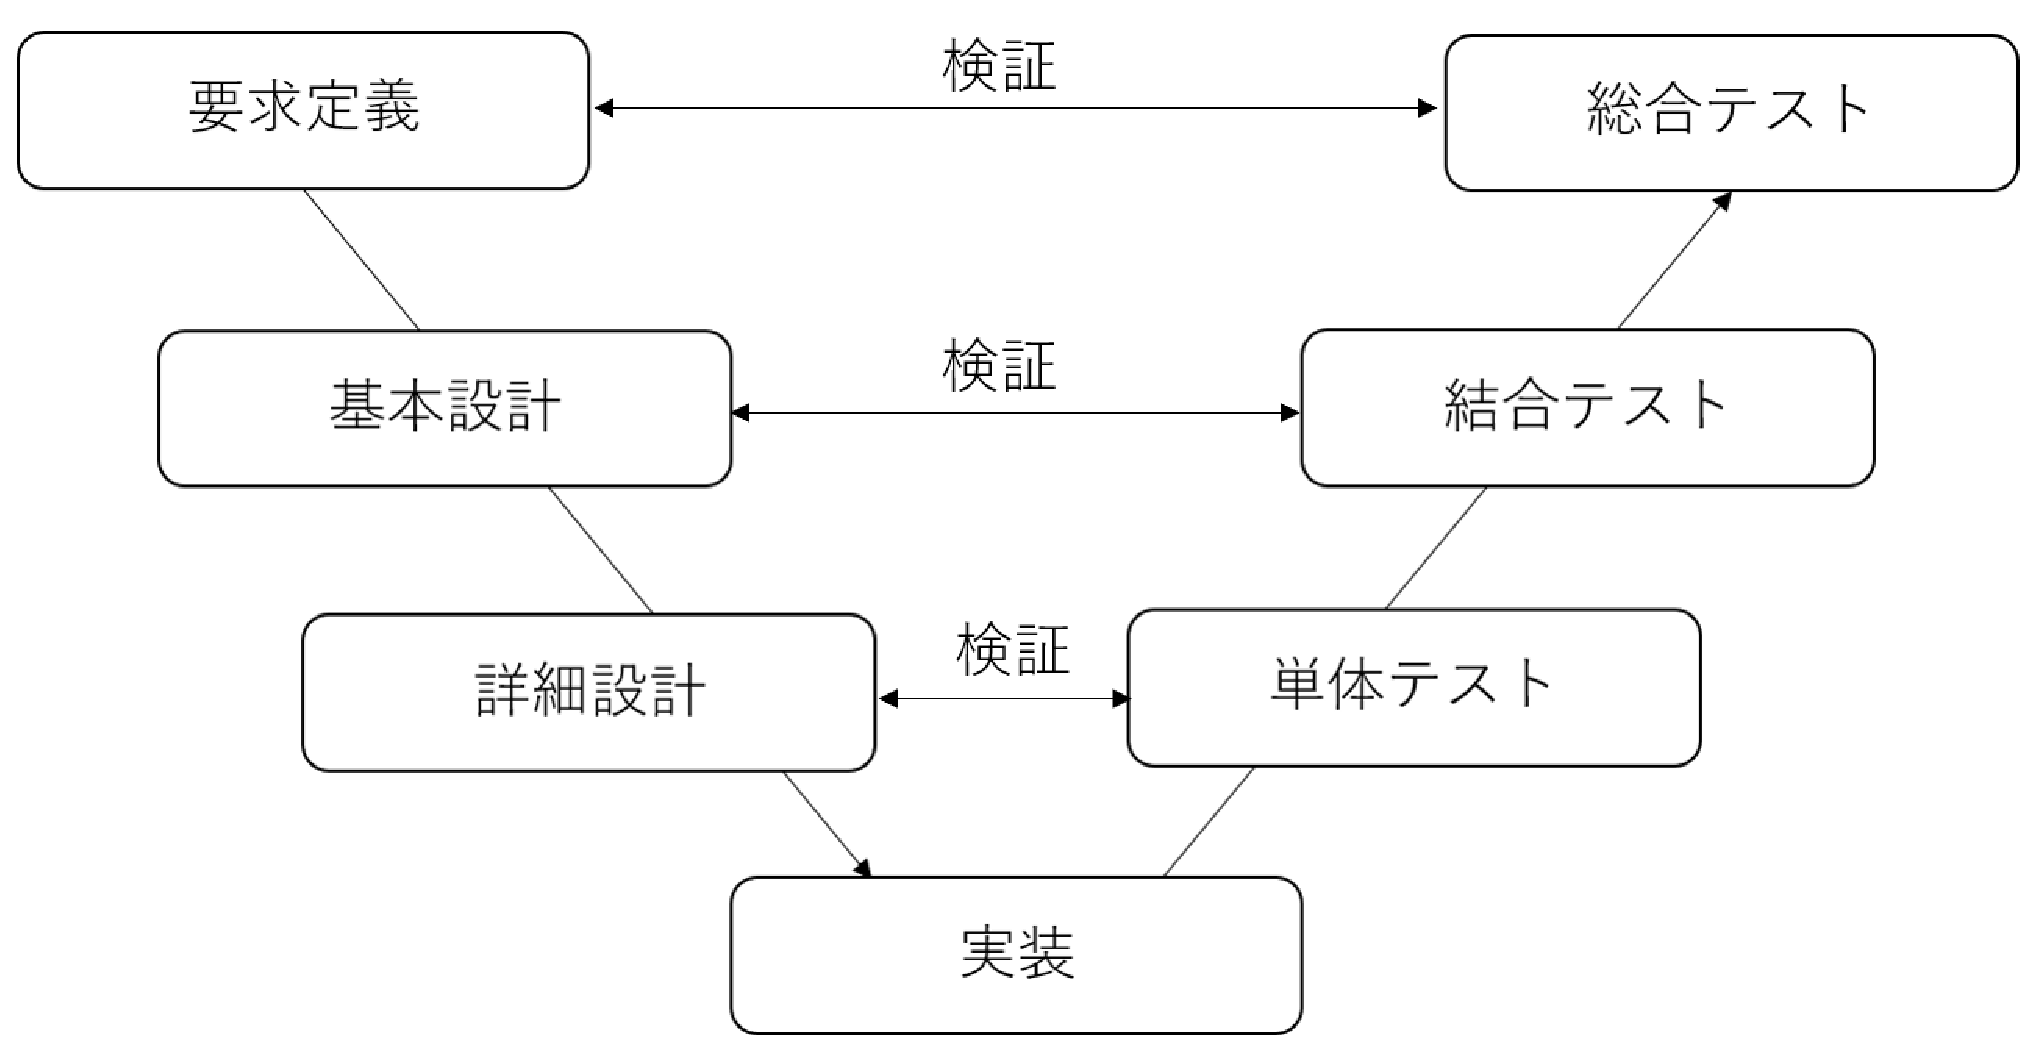
\includegraphics[width=9cm]{./vmodel2.eps}
	\caption{V字モデル}
	\label{vji}
\end{figure}


\subsection*{UML(Unifiled Modeling Language)\cite{uml}}

UMLとは統一モデリング言語(Unified Modeling Language)のことである.OMG\\(Object Management Group)と呼ばれる企業団体の標準規格として正式に承認されており,オブジェクト指向を用いている.

\subsection*{ユースケース図\cite{uml}}

ユースケース図とは,UMLで定義されている図のひとつであり,ユーザやクライアントの要求事項,システムに対して課せられている基本機能やサービス項目などの要件定義を表現するときに広く用いられる.現在考えているシステムを中心に置き,システムとその利用者(外部システムを含む)とのやりとりを表現する.利用者や外部システムをアクターとし,各アクターごとにシステムが提供する機能やサービスを識別したものをユースケースとして表現する.

\subsection*{クラス図\cite{uml}}

クラス図はUMLの基本となる図のひとつである.問題領域の構造や対象システムの静的な構成,システムの詳細設計,あるいは企業の部門の業務モデルの基本構造,問題解決の最初のとっかかりとなる概念マップの構築,といったことに広く使うことができる.クラス図を使うことで,対象システムを構成するクラス(概念や事物・事象)とそれらの間に存在する関連(意味的・物体的な繋がり)を表現できる.また,各オブジェクトがどのような属性やアクション(操作)を持っているかも合わせて記述することができる.

\subsection*{アクティビティ図\cite{uml}}

アクティビティ図とは,UMLで定義されている図のひとつであり,アプリケーションのある機能の動作の様子など,システムのワークフローを表現する.並列処理や待ち合わせ同期といった並行表現ができる.

\subsection*{シーケンス図\cite{uml}}

シーケンス図とは,UMLで定義されている相互作用図の一種であり,システムの一機能が時間経過の中でどのように動くかという動的な振る舞いを表現する.オブジェクト間のメッセージのやりとりを時系列に沿って記述するため,振る舞いを順番に追っていくのに役立つ.

\subsection*{ステートチャート図\cite{uml}}

ステートチャート図とは,UMLで定義されている図のひとつである.一つのシステムやオブジェクトのライフサイクルを状態遷移図として表現する.
	
	%第3章 
	\chapter{感染症予防サポートシステムの設計}
	%第3章
本章ではまず、3.1節にて本研究で開発する「感染症予防サポートシステム」の概要を述べる。続いて3.2節ではユースケース図、ユースケース記述を用いて、システムの要求定義について述べる。3.3節ではアクティビティ図、クラス図を用いて、システムの基本設計について述べる。3.4節ではシーケンス図を用いてシステムの詳細設計について述べる。


	%第3-1章
\section{感染症予防サポートシステムの概要}
本節では、はじめに感染症予防サポートシステムの開発の目的について説明した後、それを実現するための手段、開発を進める際の課題について述べ、実際に開発したシステムの概要について説明する。

まず私たちは、システムを開発するにあたって、本研究で開発するシステムの目的を定めるところから始めた。何よりもこのシステムで実現しなければならないことをメンバー同士で議論し合った結果、1章で述べたように、世界的な感染拡大が続く新型コロナウイルスへの感染予防対策の一環として取り組むべきとされている、3密の回避のサポートを第一の目的とした。具体的には、学校の教室などの、数人から数十人程度が利用するような部屋で稼働させることで、その部屋に入室可能な人数の目安を示し、部屋の警戒レベル・感染リスクを分析することで、密閉を防ぎつつ、状況に応じて部屋に滞在可能な人数を段階的に制限することによって、その部屋に滞在する人々を3 密の危険から守ることを想定し、システム開発を進めることとなった。続いて私たちは、この目的を実現するためにシステムが果たすべき役割として、以下の2つが挙げられると考えた。


\begin{itemize}
	\item 感染症予防対策のルールを守ってもらうよう働きかける役割
	\item 感染症予防対策の基準を定める役割
\end{itemize}

少なくともこれら2つの役割を満たして、はじめてこのシステムが利用者による3密回避のための行動をサポートできると考えた。3密の回避においては、「密閉」「密集」「密接」の3つの要素が関与することから考えても、上に示した2つの役割を果たすシステムの開発を行うには、その方法を十分に議論する必要があったが、実際の詳細な設計に関しては後で述べる。

続いて本研究で開発するシステムが、先ほど述べた2つの役割を果たすためには、どのような働きを持つべきかを議論した。

まず、利用者に感染症予防対策のルールを守ってもらう役割を果たすには、利用者の感染症予防対策への取り組みの状況を、利用者自身が把握できる必要があると考えた。つまり、リアルタイムで部屋の利用者の感染症予防対策の取り組みを監視し、現在の取り組みがルールに即したものであるかどうかの度合いを知らせ、ルールに反している場合には警告を出すなどし、利用者に感染症予防対策を促すような機能が求められると考えた。

また、感染症予防対策の基準を定める役割を果たすためには、リアルタイムな環境モニタリングによる、総合的な環境分析から得られる結果に基づいた基準を定める必要があると考えた。ここでは、環境の監視と分析の2つの機能が必要となり、環境の監視からどのような情報が得られ、その情報が分析の機能によって、どう意味付けされ、分析の結果得られる情報が感染症予防対策に、どう反映されるべきかを考える必
要がある。

このように、本研究で開発するシステムには、監視と分析という2つの機能が必要になる。これらの機能について、機能を実現する際の方針と課題について述べる。

\subsubsection*{監視の機能}

まず監視の機能については、どのような情報をどのようにして収集するかを考えた。まず3つの密のうち、「密閉」を避けるためには部屋の換気状況を監視する必要がある。こちらは、部屋に人が滞在している状況で、部屋の空気の入れ替えが十分に行われているかどうかを把握できれば良いため、室内の二酸化炭素濃度の高さを監視することによって、状態を把握できると考えた。

ここで考慮しなければならないのが、適切に部屋の換気状況を調べるためには、どのような場所に何台のセンサデバイスを設置すればよいかである。二酸化炭素は気体の一種であるため、部屋中に一様に広がっているわけではなく、同じ部屋の中でも場所によって、微妙に濃度が異なるはずである。したがって、部屋の中心に1台のセンサデバイスを設置しただけでは、室内の二酸化炭素濃度を適切に計測したことにはならないため、部屋の広さに応じてセンサデバイスを、複数台設置する必要があると考えた。ただし、ここで用いるセンサデバイスには、1章でも述べたように無線マイコンモジュールTWELITEを選定した。

「密集」「密接」を避けるためには、部屋に滞在する人の数を監視するだけでなく、部屋の広さに関する情報も必要となると考えた。また、ソーシャルディスタンスを保つために、何平方メートルに1人が滞在可能とするかといった、部屋の運用ルールも併せて考えることが、「密集」「密接」の回避のために扱う情報として適当であると考えられることから、部屋に関する情報も併せて分析の対象とすることとした。

部屋に滞在する人の数に関しては、室内にWebカメラを取り付けたマイコンを設置し、取得した室内画像に対し、物体検出の技術を用いることで、監視することが可能となる。ここで考慮すべき点は、Webカメラによって部屋全体の画像を取得するには、どのようにマイコンを設置しなければならないかという点と、画像識別のプログラム実行にかかる時間によって、監視のリアルタイム性が損なわれないかという点である。今回採用した物体検出の技術による人数推定の方法では、Webカメラによって取得する室内画像が室内全体を捉えていなくてはならない。本システムで想定している利用環境は、学校の教室などであるため、部屋の前方の壁に取り付けるのが、最も部屋全体を捉えるためには適している。反対に、部屋全体を捉えられるような場所にカメラを設置できない場合や、部屋が広すぎるために1台のカメラでは部屋全体を捉えられないという場合には、本システムの運用には適さないということになる。

なお、本システムにおける、物体検出技術による人物の検出機能には、検出精度のみならず、迅速に人物検出の結果を出力することが求められることから、GPUによる高速な処理を可能とする高価なマイコンが必要となる点や、複数箇所から撮影した複数枚の画像から、室内の人数を推定することの技術的な壁の高さから、Webカメラとマイコンの対を、1つの部屋に複数設置するということを本研究では行わない方向となっている。このような点から、本システムを運用する際に推奨される環境としては、数人から数十人程度で使われる、比較的小さな部屋で、なおかつ設置したカメラによって部屋全体を撮影できることが条件となる。ただし、ここで用いるマイコンには、1章でも述べたようにAIエッジ向けコンピュータとして知られるJetsonシリーズのJetson nanoを選定した。

\subsubsection*{分析の機能}

分析の機能に関しては、監視によって得られた情報から、より高い価値を持つ「感染予防対策に役立てられる情報」を導き出すための分析方法を議論した。

分析の機能でははじめに、二酸化炭素濃度の高さから、部屋の感染症に対する警戒レベルを導出する。二酸化炭素濃度が高くなるほど、部屋が密閉された状態になっていると考えられるため、部屋の警戒レベルは高く設定される。ここで考慮しなくてはならないのが、ある時間に取得した二酸化炭素濃度だけで部屋の換気状態を正しく分析できるかという点であり、データに多少のばらつきがみられる可能性から考えて、一定時間連続的に取った値をもとにして分析を行う必要があると考えた。

続いて、導出された警戒レベル毎に制限される、室内に滞在可能な人数と、実際に室内に滞在している人数とを比較し、感染リスクを導出する。警戒レベル毎の滞在可能人数には、上限と下限を設け、上限を超える場合には感染リスクが最高となり、下限から上限の範囲内であれば、室内の滞在人数を維持できるものとし、下限を下回る場合には、感染リスクを高めない範囲内で滞在人数を増やすことができる段階にあるものとして、3段階で感染リスクを評価する。ただし、警戒レベルの高さに関わらず、部屋の広さと部屋の運用ルールから求められる部屋の滞在可能規定人数を上回る場合には、感染リスクは最高となる。

このようにして、分析の機能では、室内環境の監視によって得られた情報をもとに、部屋の警戒レベルと感染リスクを評価する。

ここまで、本研究で開発するシステムの目的、機能を実現する際の方針と課題について述べてきた。ここからは、実際に開発したシステムの概要を説明する。

まず、本研究で開発するシステムを利用する際の簡単な流れを図\ref{systemflow}に示す。

\begin{figure}[H]
	\centering
	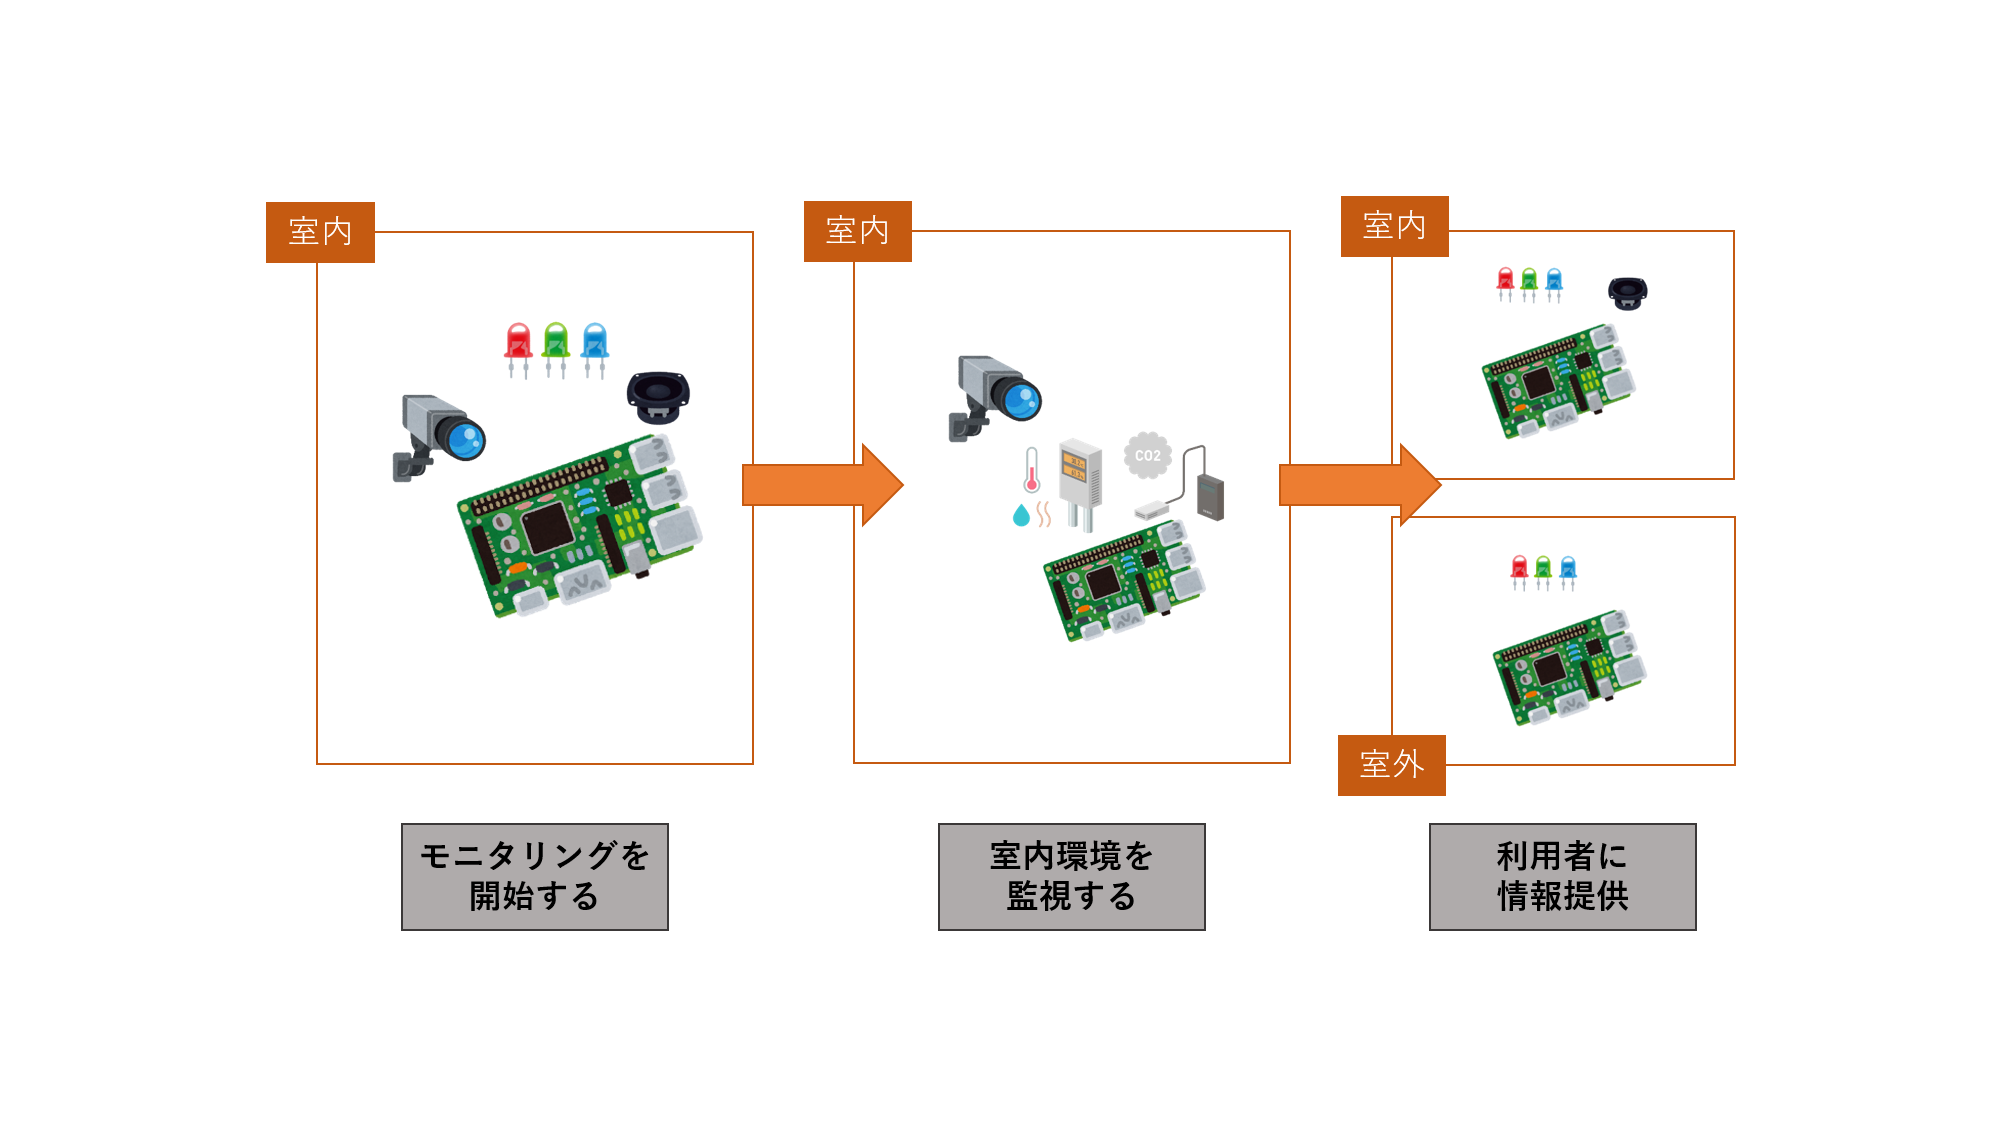
\includegraphics[width=15cm]{systemflow.eps}
	\caption{システム利用の流れ}
	\label{systemflow}
\end{figure}

まず、利用者はエッジサーバとしてシステム全体の中心となって稼働するJetson nanoに、部屋情報として、部屋の広さと何平方メートルに1人が滞在できるかという、部屋の運用ルールを登録する必要がある。感染予防サポートシステムを稼働させるには、このJetson nanoと、センサデバイスとして用いるTWE-LITEを室内に設置する。センサデバイスは部屋の広さなどに応じて、台数を増やすことが可能である。また室外には、部屋への入室の危険度を知らせるためのデバイスとして用いるTWE-LITEを設置する。あとは各デバイスの電源を入れ、エッジサーバであるJetson nanoによってモニタリングを開始するのみである。

デバイス類はシステム稼働後にそれぞれ接続され、基本的には3分おきに室内画像と、二酸化炭素濃度や温湿度といった環境値をそれぞれ、Jetson nanoに取り付けたWebカメラ、室内センサデバイスに取り付けたセンサ類によって取得し、それらのデータをJetson nanoで受け取った後、室内画像をもとにした人数推定と環境値をもとにした分析を行う。Jetson nanoでは、分析結果に基づき、換気要請や感染リスク状況をブザーとLEDを用いて、室内の利用者に通知する。また室外デバイスでは、Jetson nanoにより分析された部屋への入室危険度を受け取り、その都度リスクに応じたLEDを点灯する。これら一連の流れを8時から20時まで行い、夜間はスリープ状態に入るというのが、基本的なシステムの稼働の流れである。ここでシステム全体構造のイメージを図\ref{systemconst}に示す。

\begin{figure}[H]
	\centering
	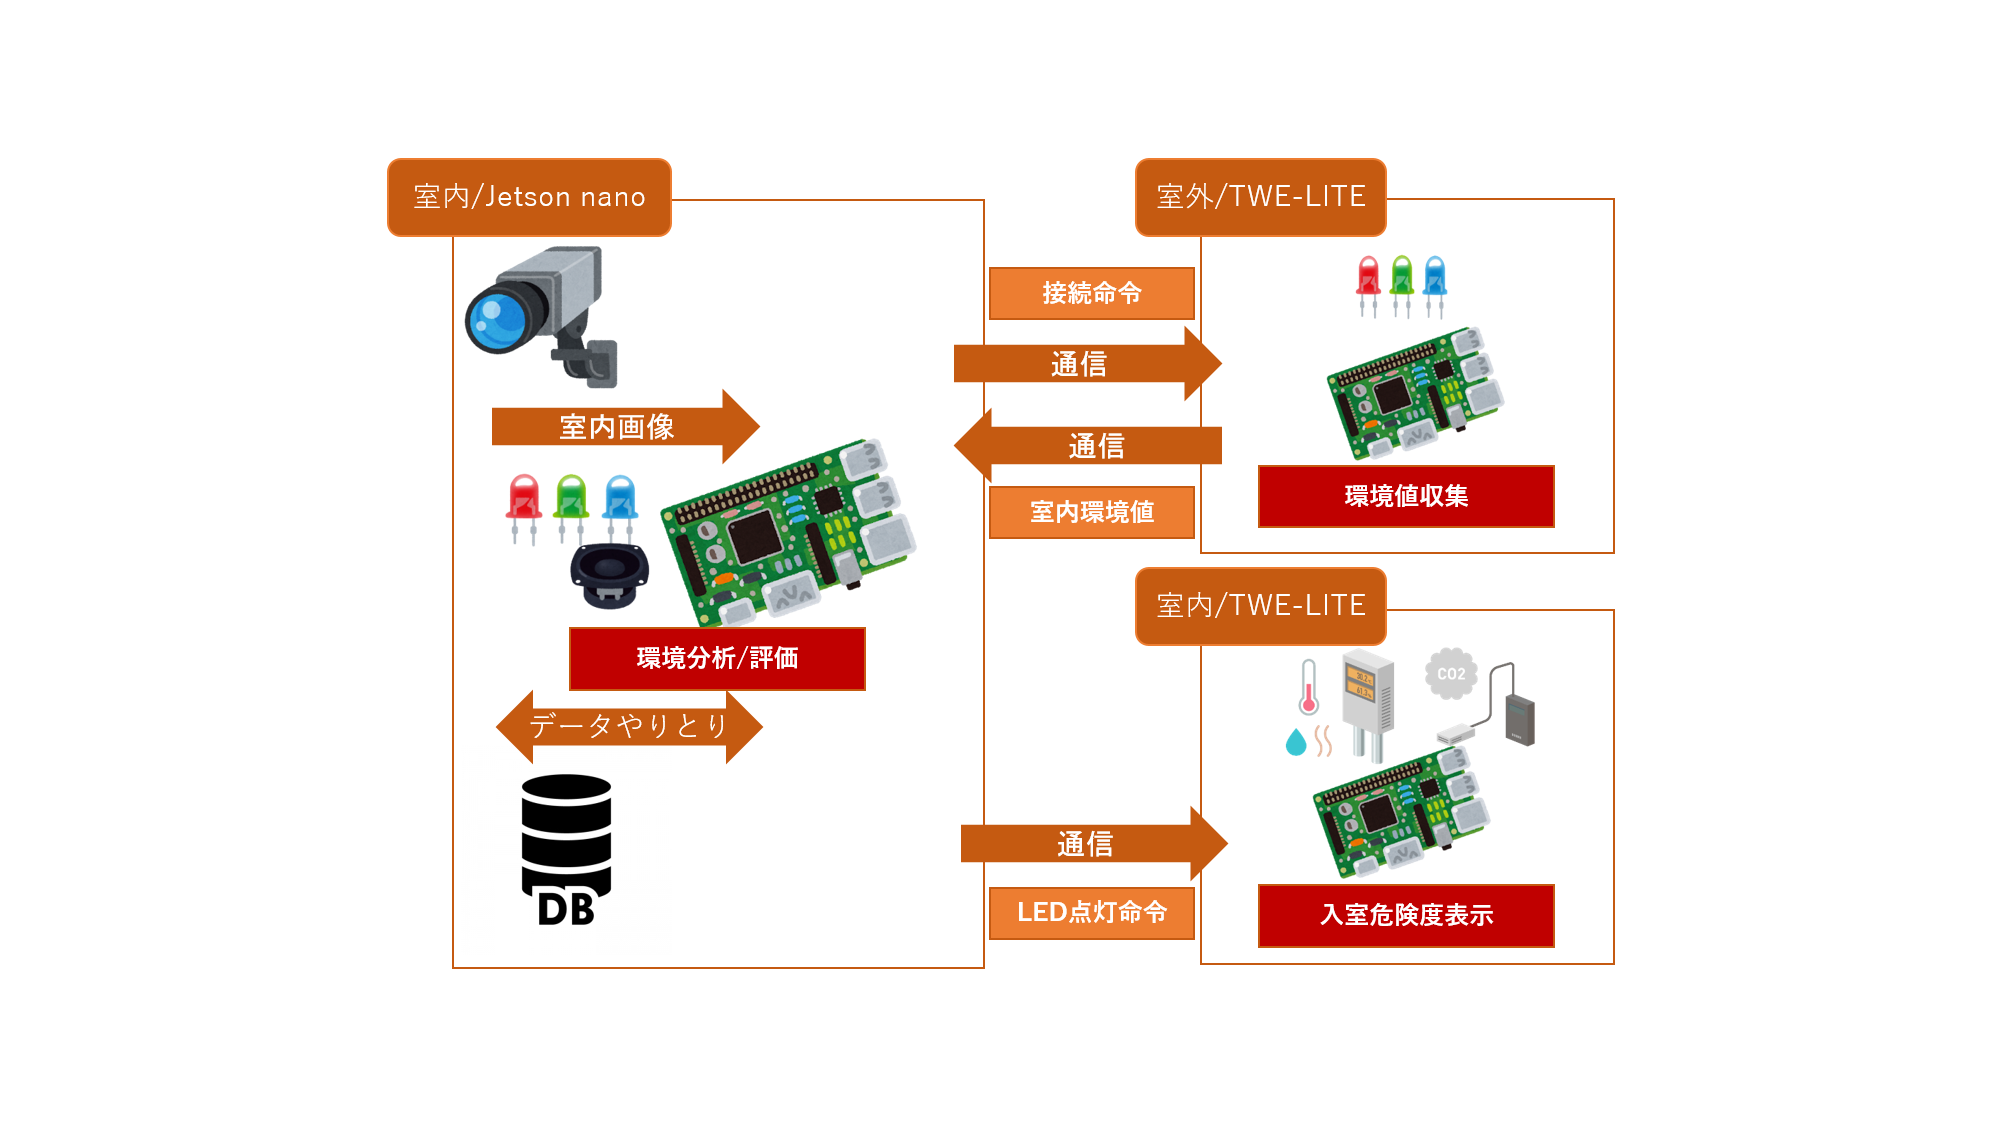
\includegraphics[width=15cm]{systemconst.eps}
	\caption{システム全体構造}
	\label{systemconst}
\end{figure}

なお本システムの開発は、エッジサーバ側を掛水誠矢が、センサデバイス側を稲田一輝が、室外デバイス側を小田恵吏奈が、人数推定機能を伊藤大輝が担当する。




	%第3章

\section{要求定義}

感染症予防サポートシステムがどのような機能を持ち,どのような振る舞いをするかを表すために以下の図\ref{usecase1}に示すユースケース図を作成した.

\begin{figure}[htbp]
\centering
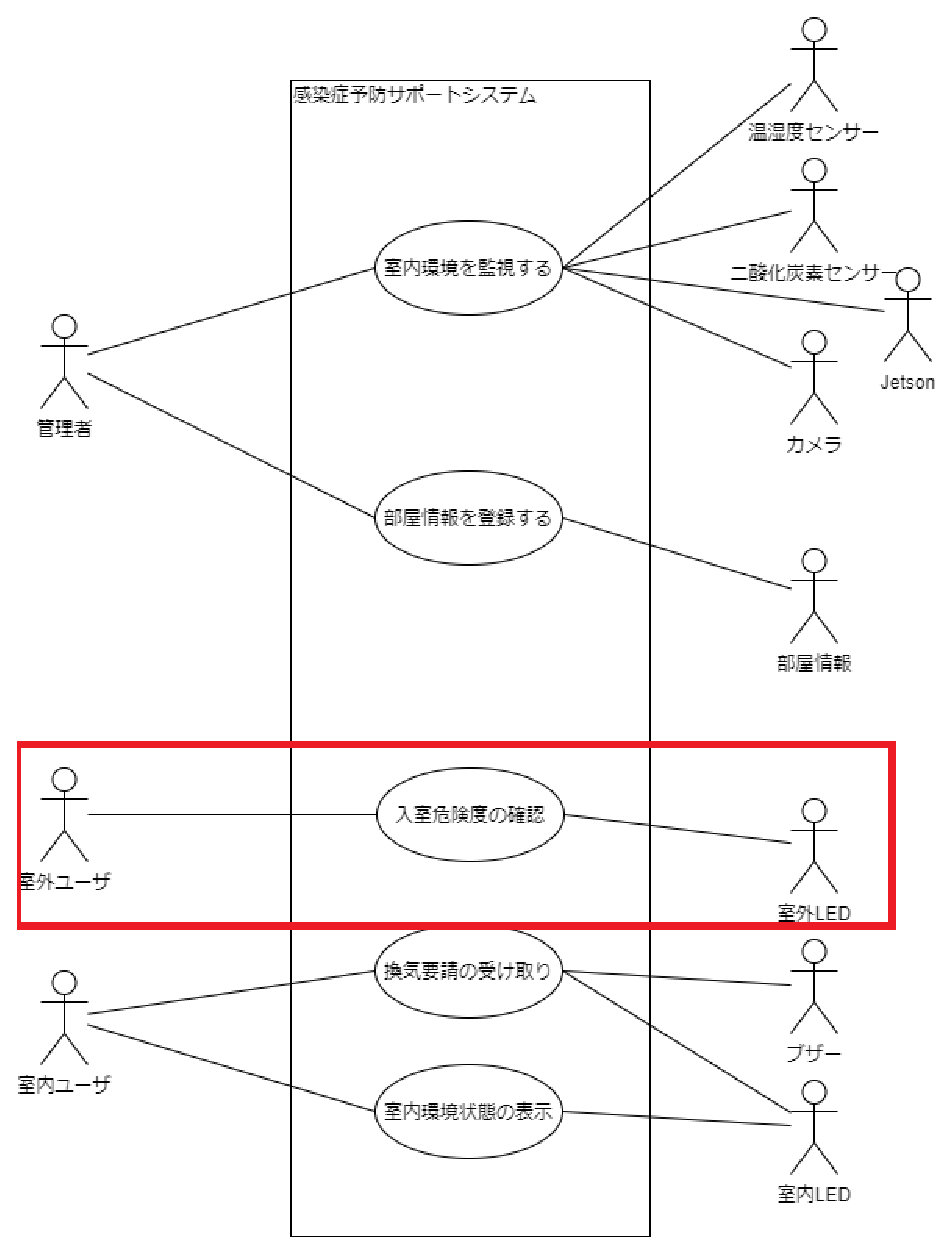
\includegraphics[width = 10cm]{./uml/usecase_e.eps}
\caption{ユースケース図}
\label{usecase1}
\end{figure}

感染症予防サポートシステムの各ユースケースについて述べる.
「室内環境を監視する」では,Webカメラにより取得した画像について人数推定を行い,室内人数に応じた監視モードを開始する.監視モードで測定した二酸化炭素濃度に応じて警戒レベルを設定し,必要に応じて換気要請を出すなどの対応をとる.
「部屋情報を登録する」では,管理者が登録した,システムを運用する部屋の広さを元に,標準警戒レベルでの滞在可能上限人数を定める.
「入室危険度の確認」では,部屋の滞在可能上限人数と現在の室内人数に応じた入室危険度を表す室外デバイスのLEDを点灯する.
「換気要請の受け取り」では,二酸化炭素濃度が各警戒レベルでの基準値を一定時間連続で超えると,LEDやブザーによって換気要請が出され,室内のユーザーは要請に従い換気を行う.
「室内環境状態の表示」では,温湿度の一定時間ごとの測定値を元に室内環境を分析し,温湿度が基準値を超えている場合は室内のLEDが点灯する.これを受けた室内のユーザーは,エアコン等により温湿度の調整を行う.
特に赤枠で囲んだ「入室危険度の確認」は筆者が実装を担当する部分となる.

上記のユースケースを受け,表\ref{sougoutestkoumoku}に示す総合テストの項目を挙げた.

\begin{table}
	\centering
	\caption{総合テスト項目}
	\label{sougoutestkoumoku}
	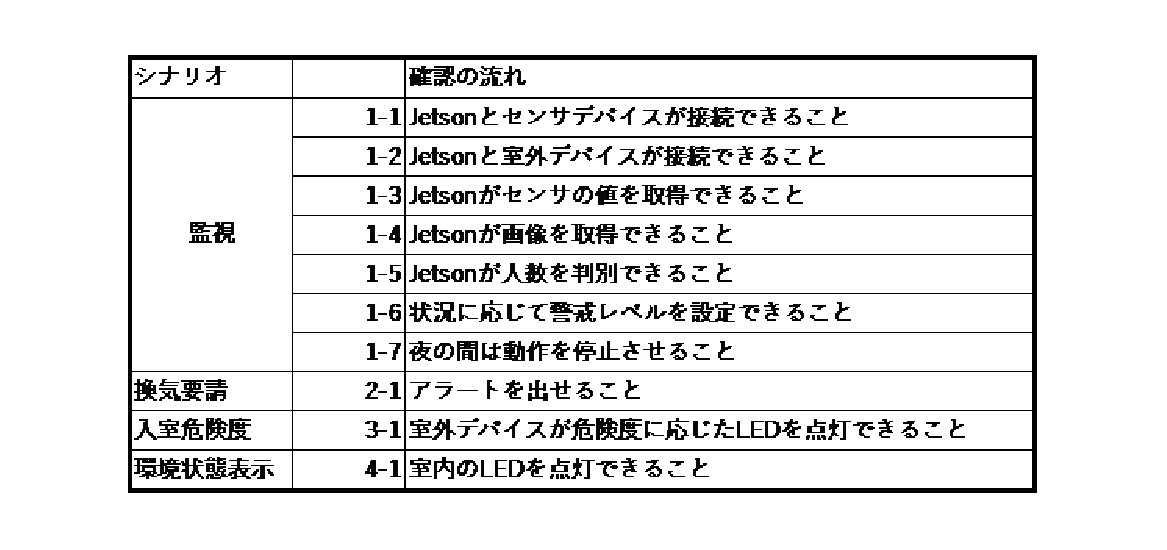
\includegraphics[width=0.9\linewidth]{test/sougoutest_koumoku}
\end{table}
\newpage
	%第3-3章
\section{基本設計}
基本設計では、ひとまとまりの処理の内容の流れを表現するために用いるアクティビティ図を作成し、「室内環境を監視する(図\ref{a_kansi})」、「換気要請の受け取り(図\ref{a_kanki})」、「入室危険度の確認(図\ref{a_nyuusitu})」、「室内環境状態の表示(図\ref{a_situnaikankyou})」の4つのユースケースについて、簡単に処理の流れを確認した。以下に作成したアクティビティ図を示す。


\begin{figure}[H]
	\centering
	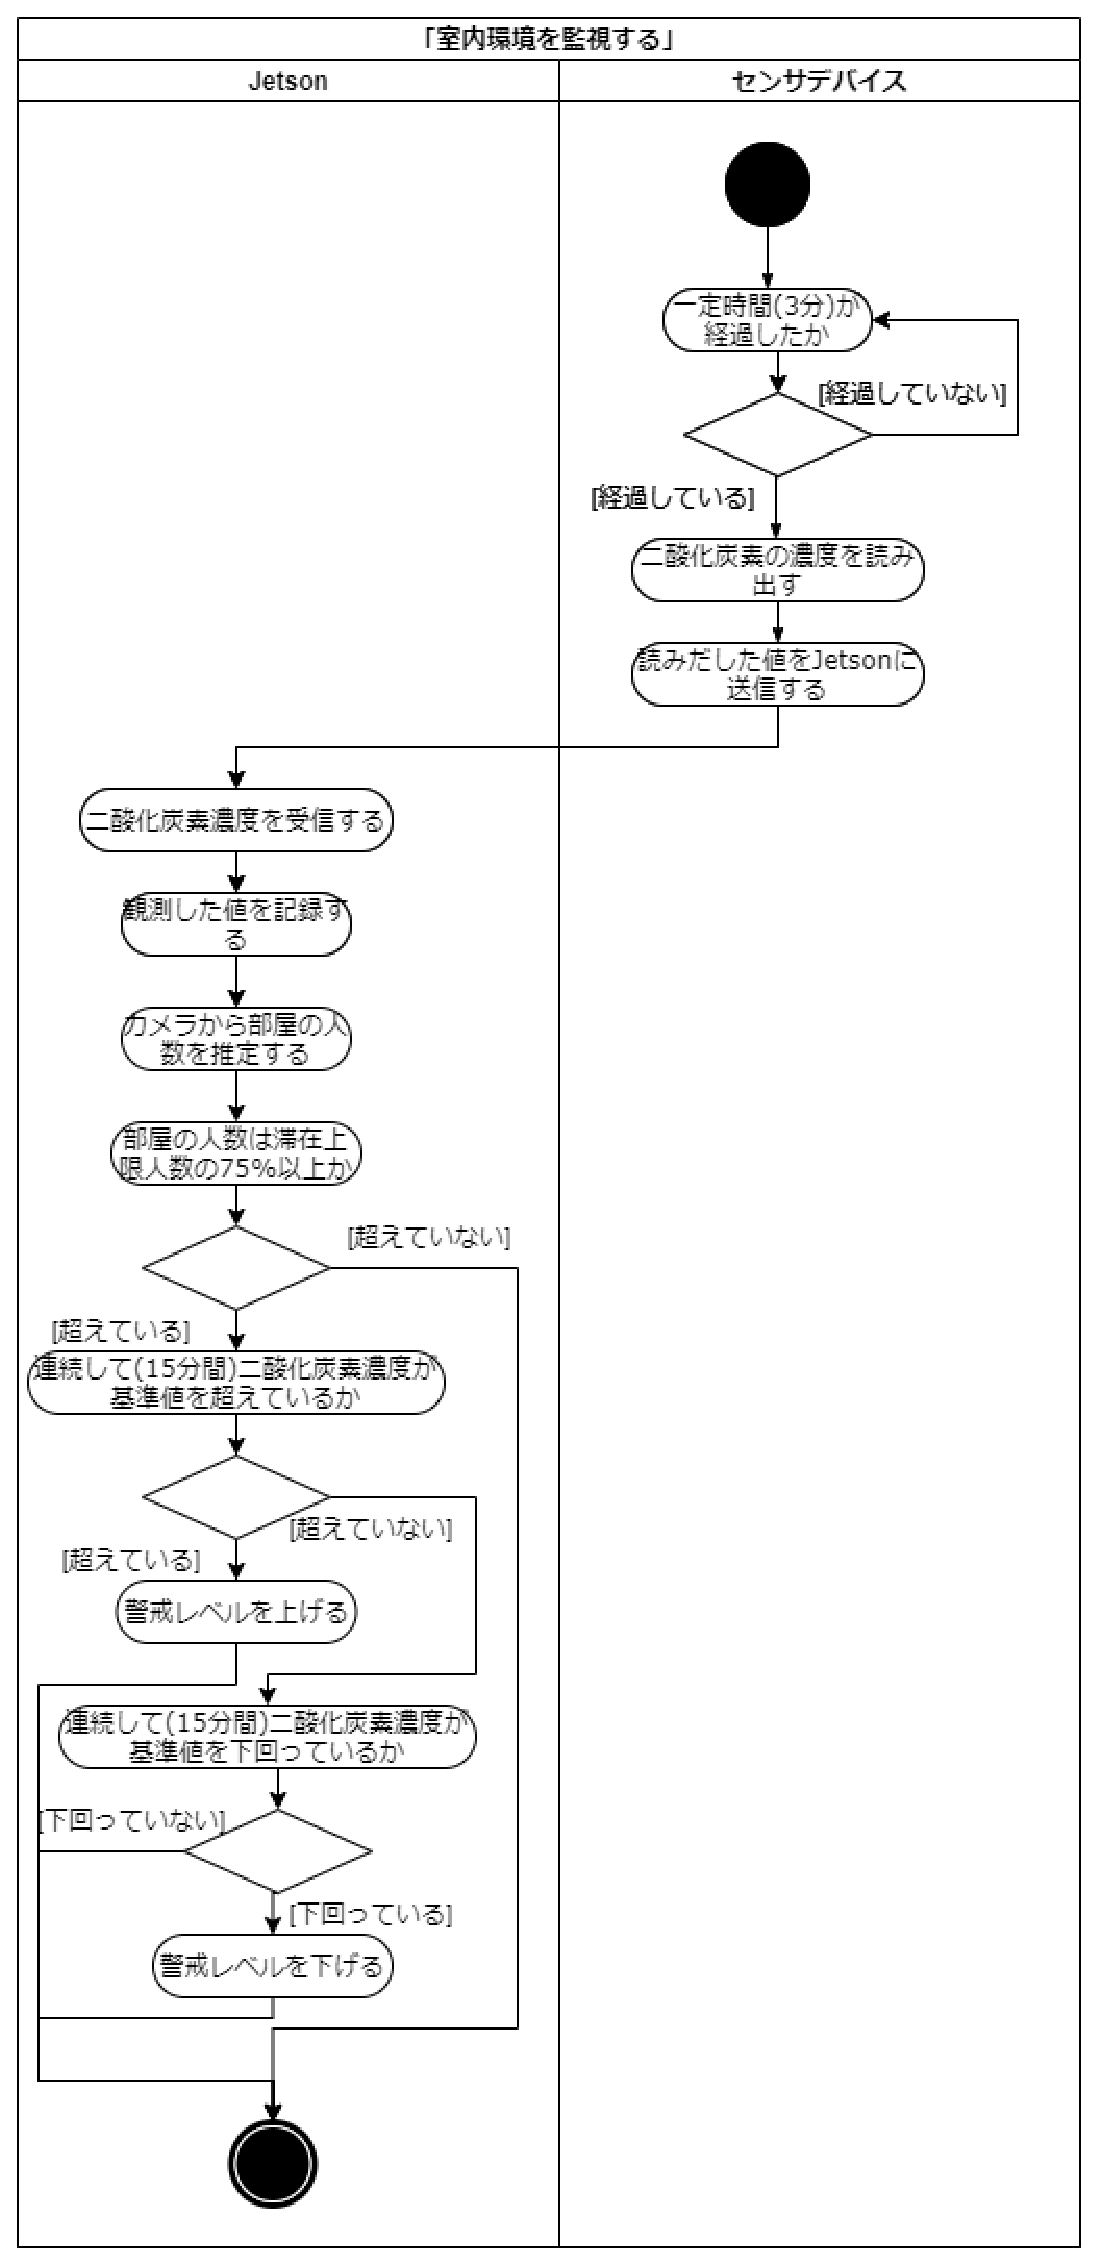
\includegraphics[width=9.5cm]{a_kansi.eps}
	\caption{室内環境を監視する}
	\label{a_kansi}
\end{figure}

\begin{figure}[H]
	\centering
	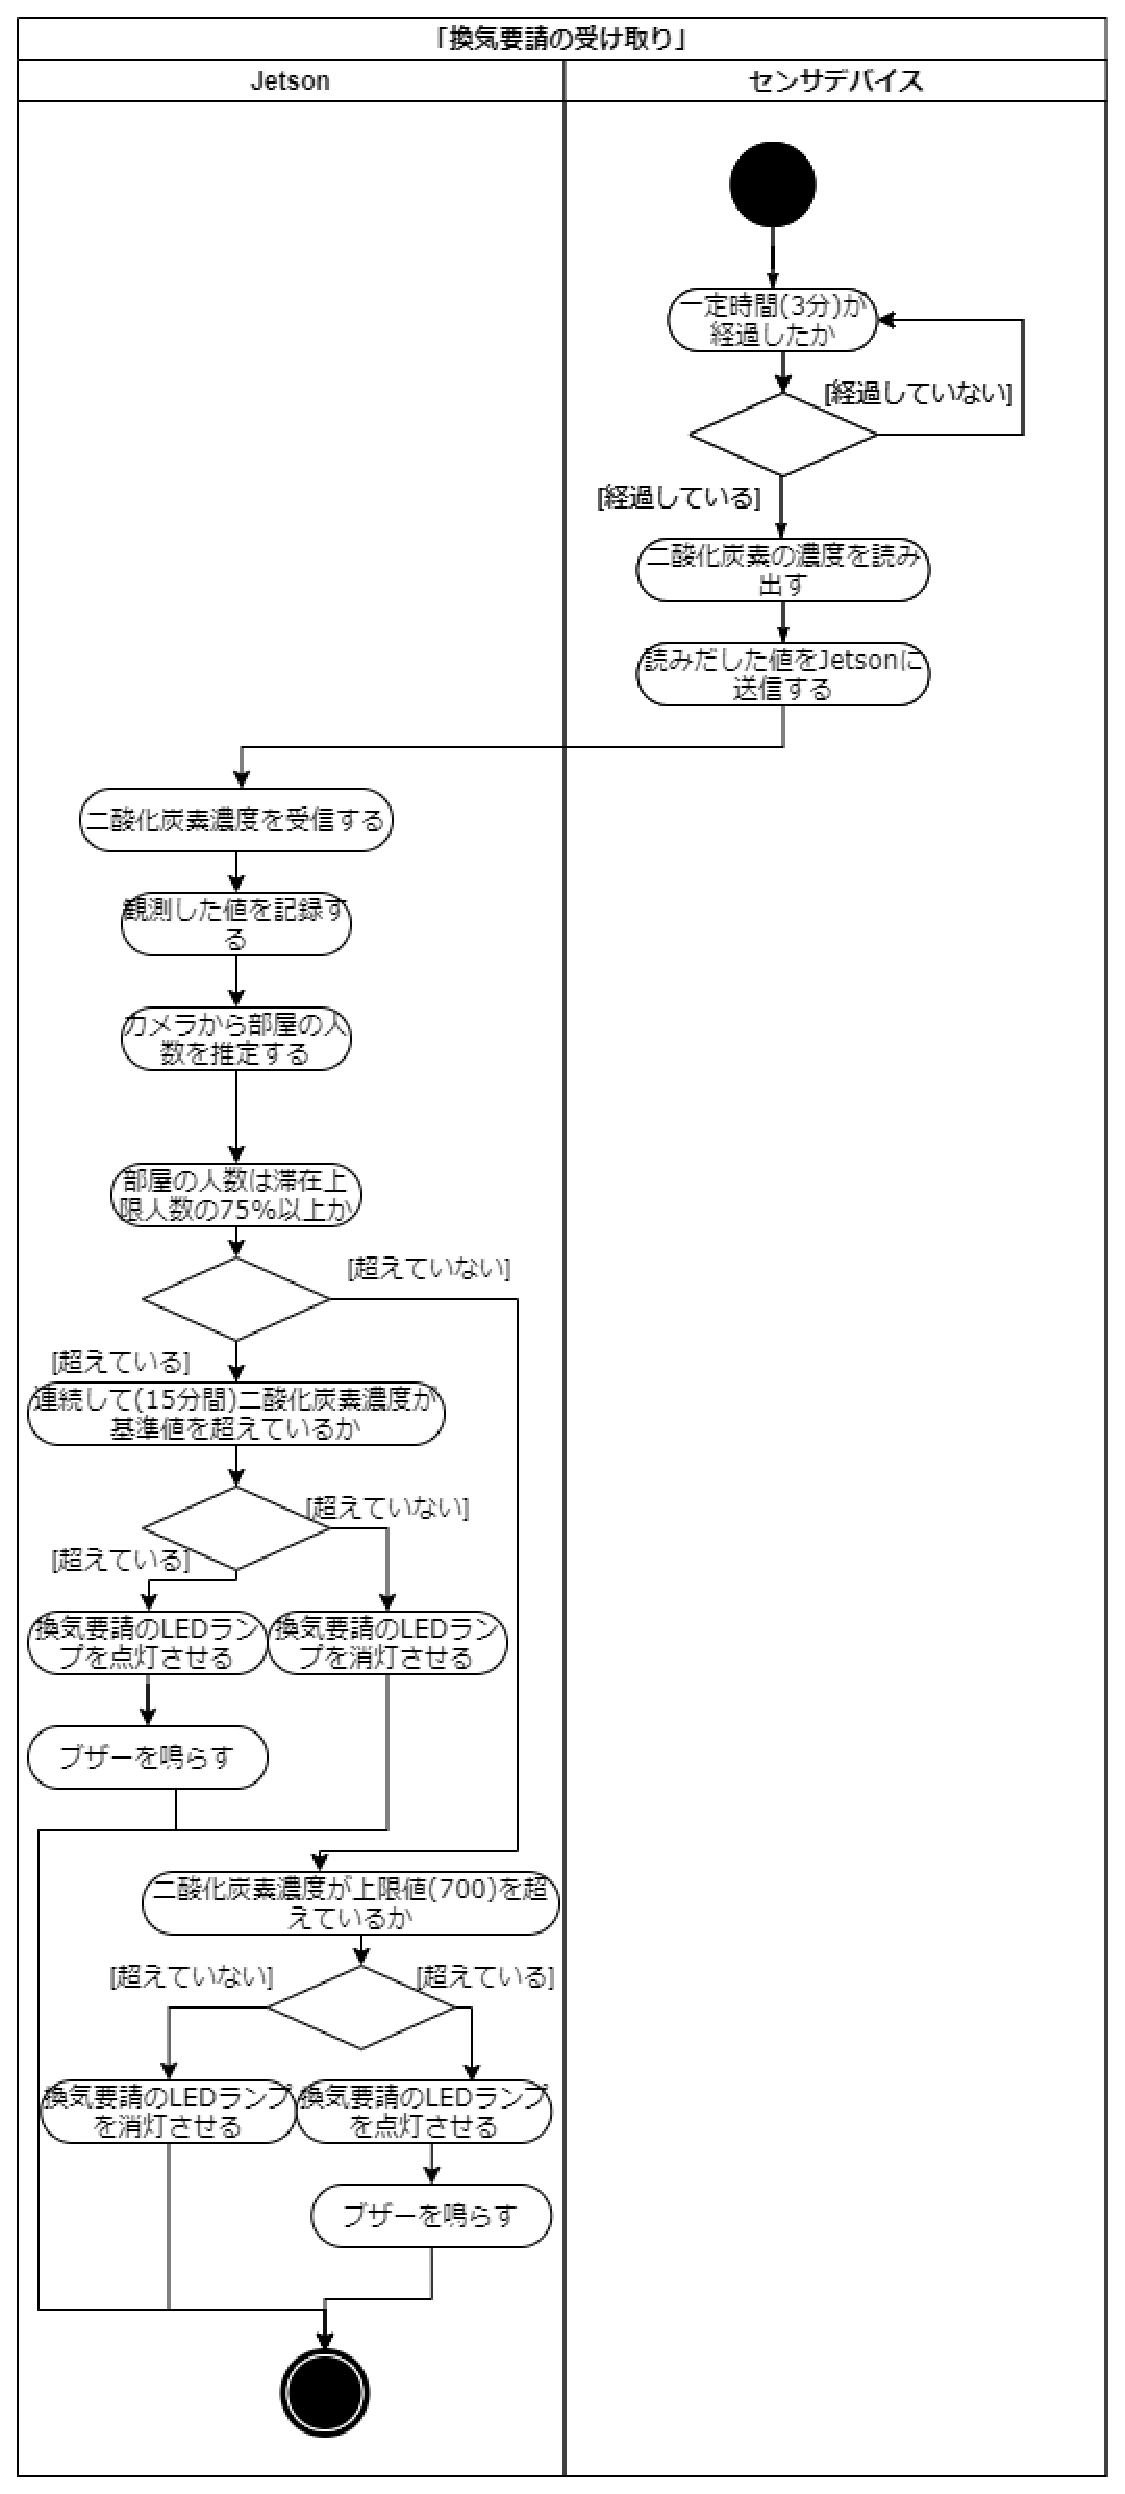
\includegraphics[width=9.0cm]{a_kanki.eps}
	\caption{換気要請の受け取り}
	\label{a_kanki}
\end{figure}

\begin{figure}[H]
	\centering
	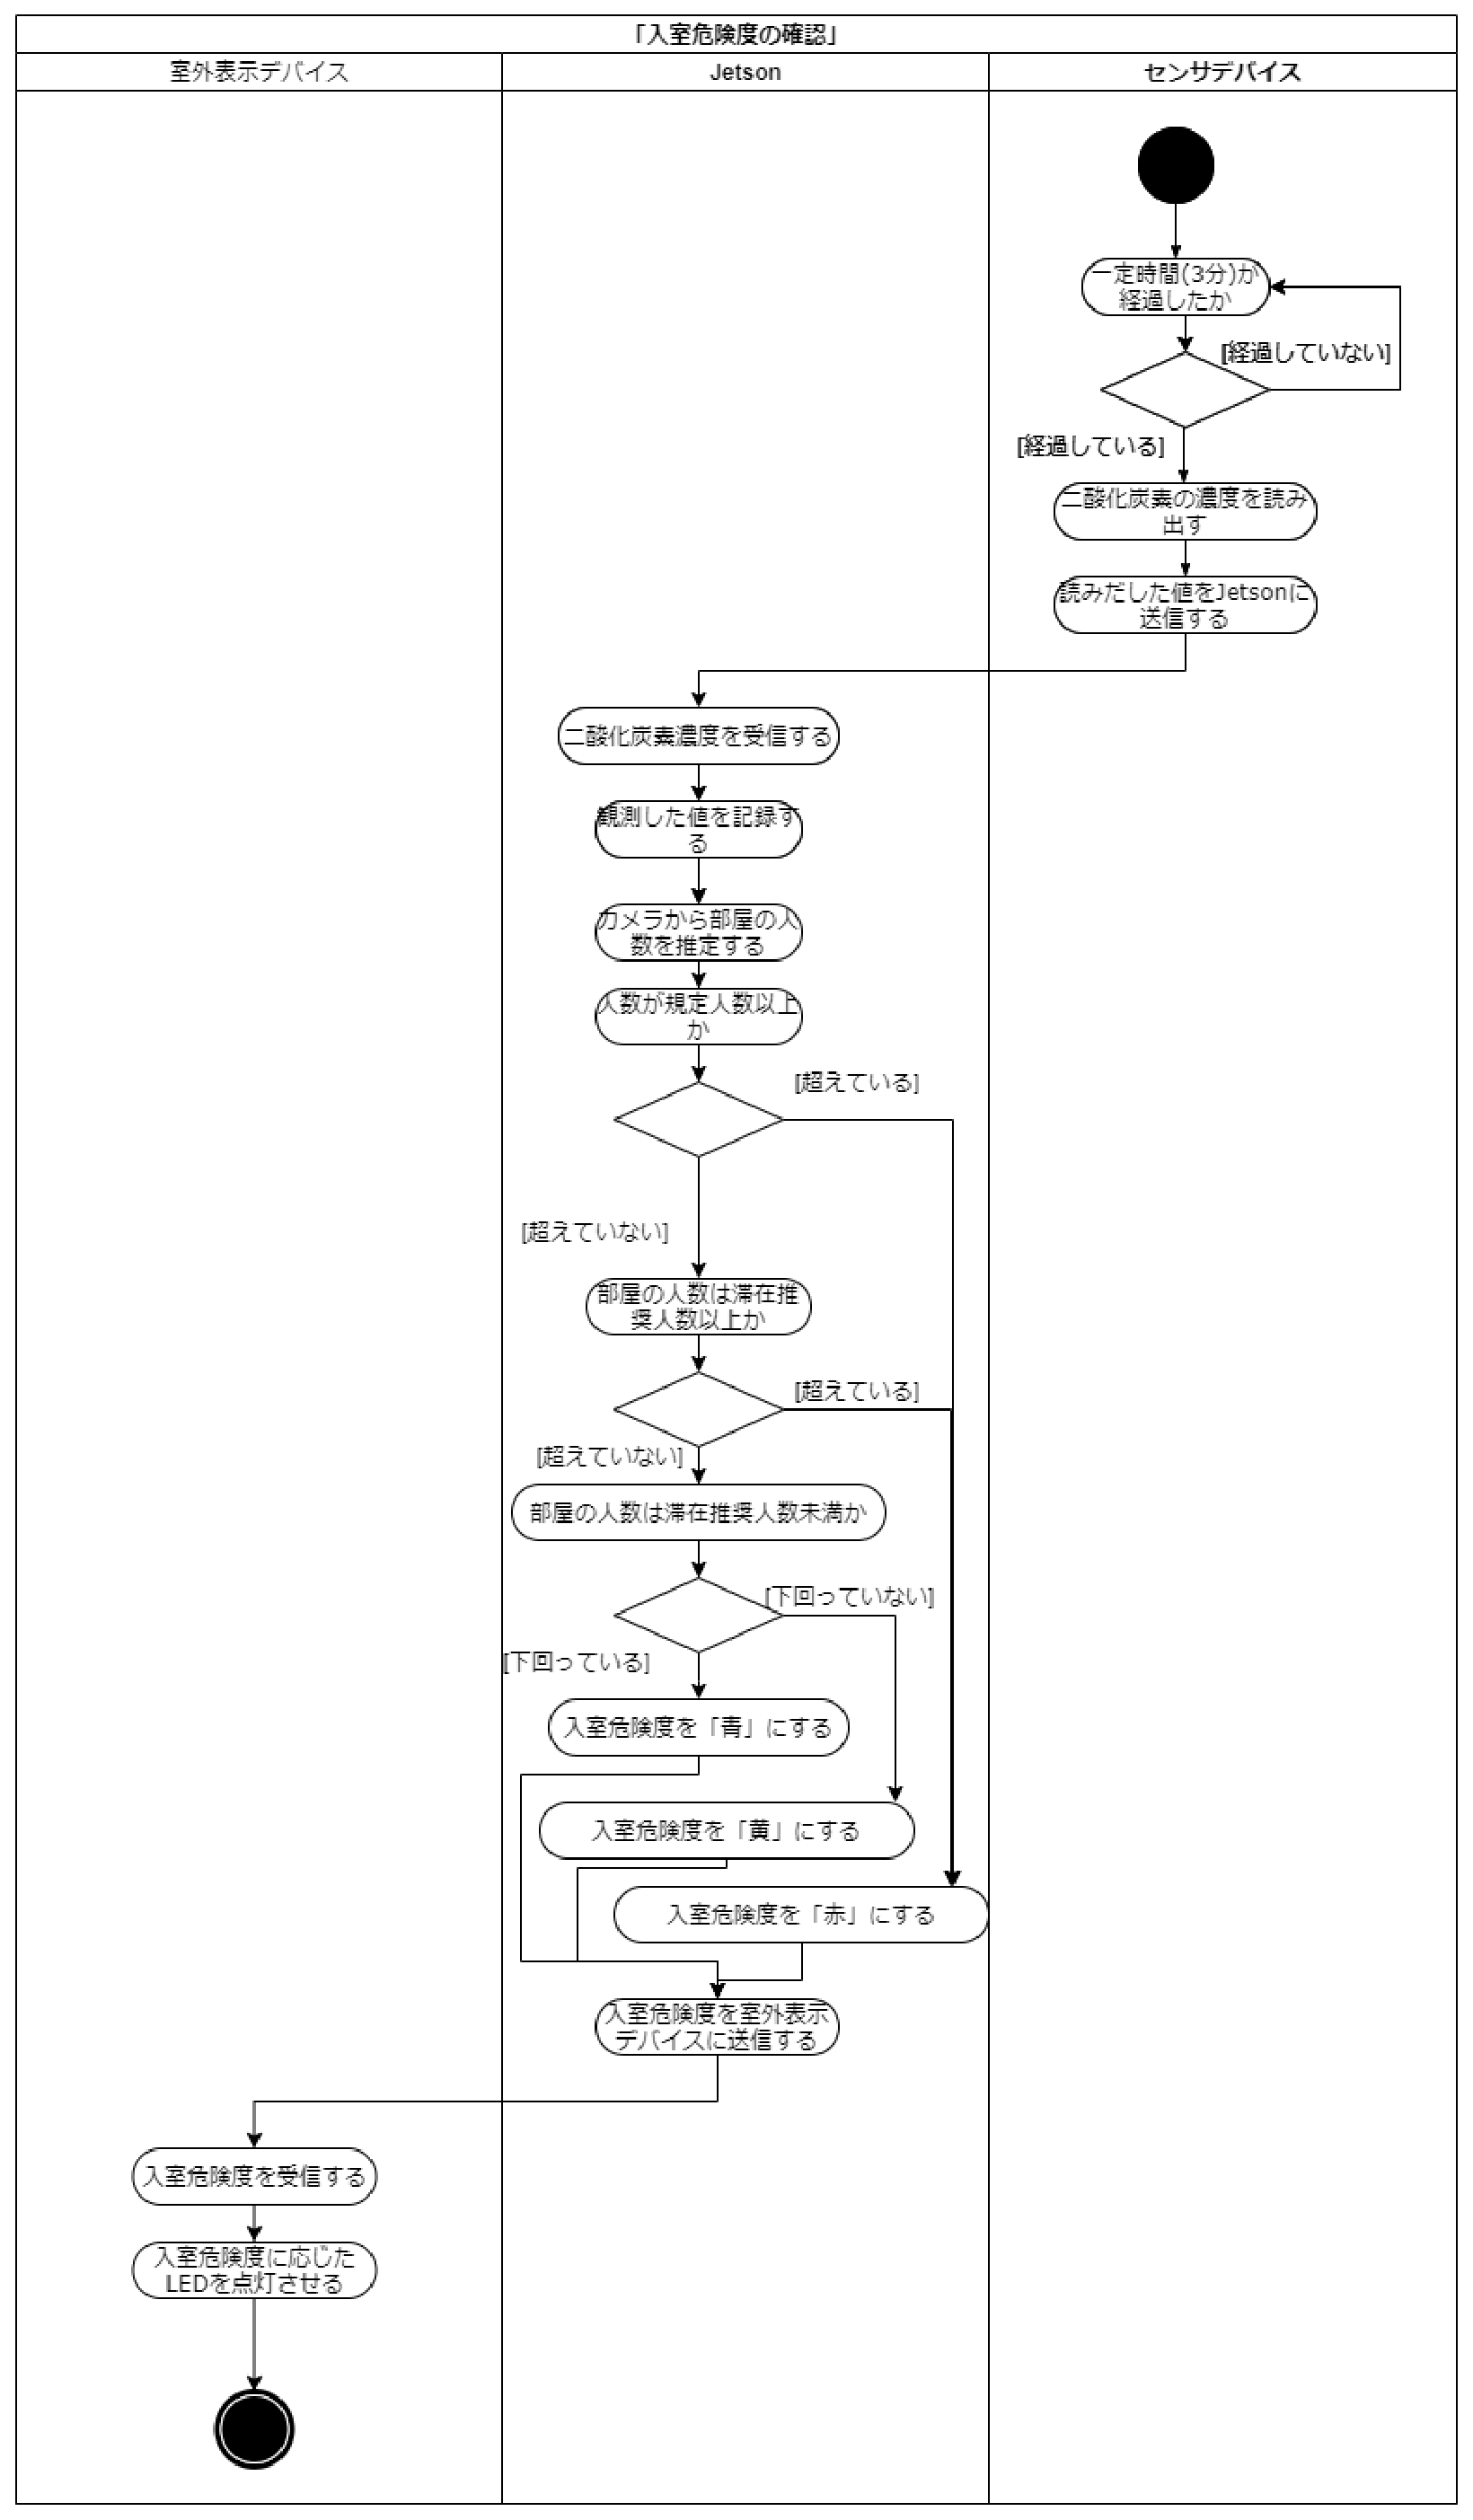
\includegraphics[width=9.5cm]{a_nyuusitu.eps}
	\caption{入室危険度の確認}
	\label{a_nyuusitu}
\end{figure}

\begin{figure}[H]
	\centering
	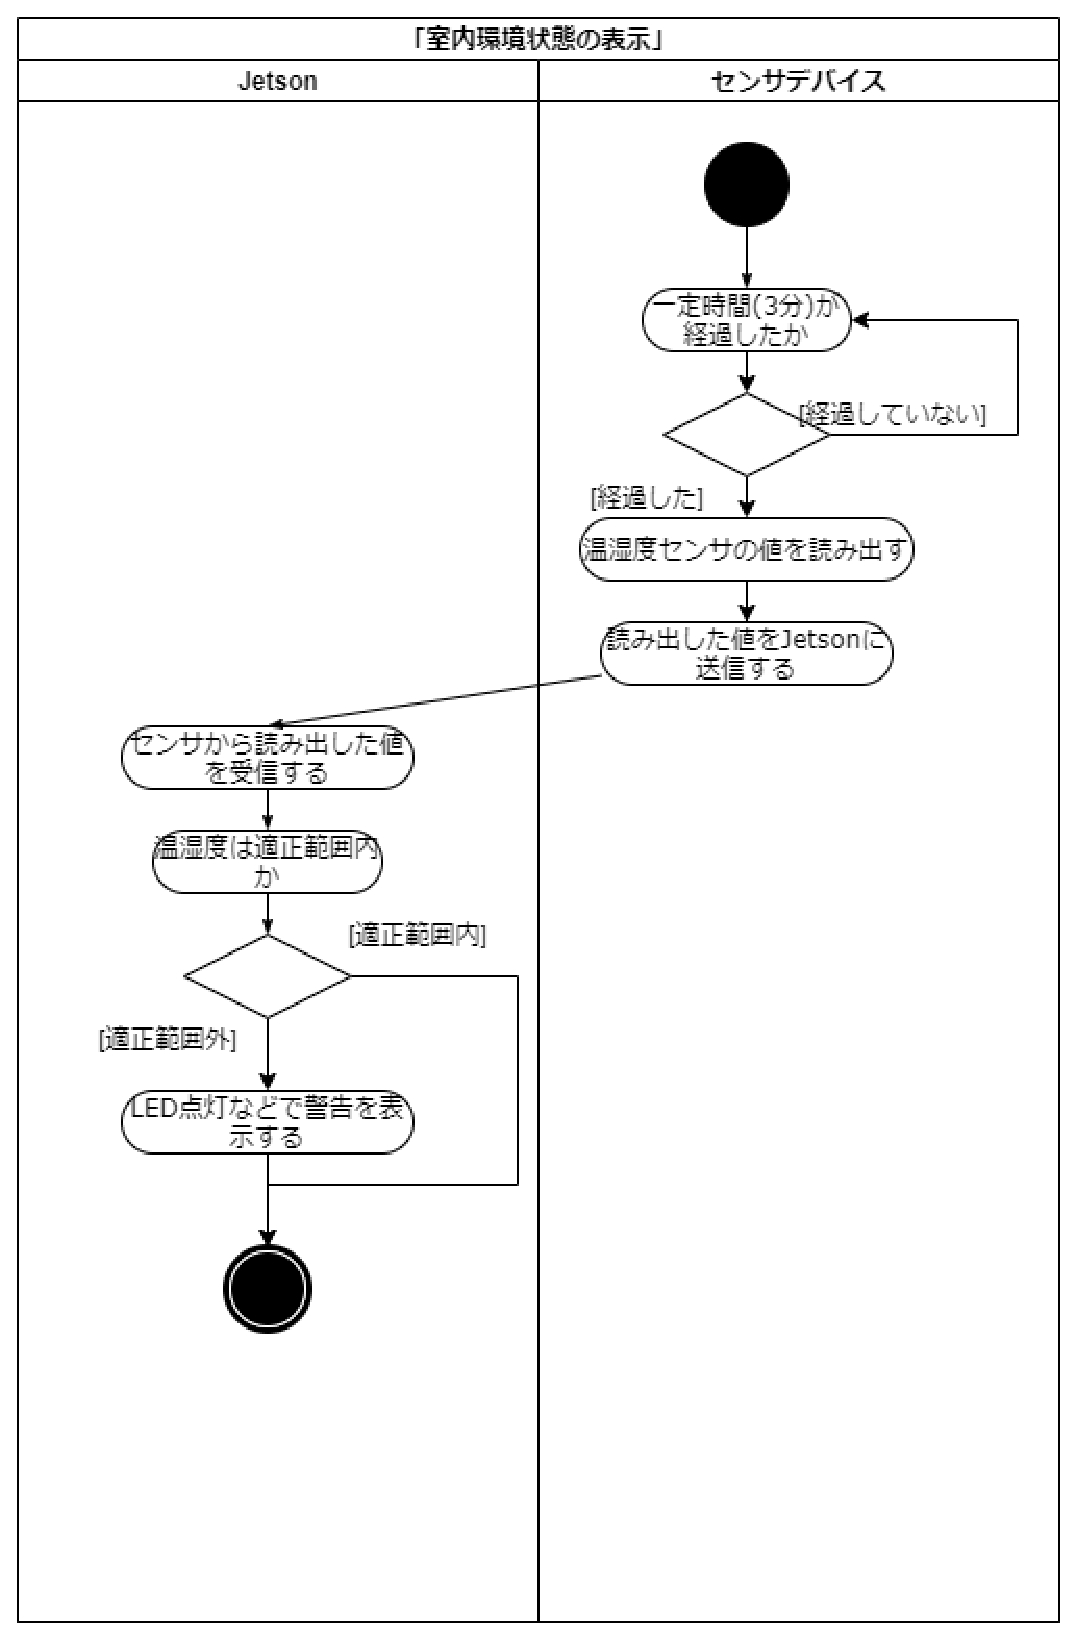
\includegraphics[width=10cm]{a_situnaikankyou.eps}
	\caption{室内環境状態の表示}
	\label{a_situnaikankyou}
\end{figure}

以上の4つのアクティビティ図の作成を通して、それぞれのユースケースを実現する際の処理の流れを可視化することができた。この作業を通して、ユースケース図やユースケース記述を作成した時点よりも、より論理的にシステム内部の設計を進めることができた。

上に示したアクティビティ図では、各デバイスなどのオブジェクトごとの処理のまとまりを、縦の線によってレーンとして明示的に分けて表現している。これによって、各ユースケースの全体的な処理の流れだけでなく、各ユースケースにおいて、処理やデータがオブジェクト間でどのように移されるかを確認することもできた。

具体的に見てみると、室内の複数箇所に設置するセンサデバイスは、センサから値を取得した後は、送信の機能を基本として動作すればよいことが確認できた。一方、Jetson nano側に着目すると、センサデバイスからのデータの受け取りと、室外の入室危険度表示デバイスへのデータの受け渡しというデータの流れが必要となることが確認され、Jetson nano側ではデータの送受信両方の役割を持たせなければならないことが確認できた。また、室外の入室危険度表示デバイス側は、データの取得・分析後の成果物の情報といえる、入室危険度の受け取りさえできればよいということから、受信の機能を基本として動作すればよいことを確認することができた。

アクティビティ図作成の段階では、まだ詳細な処理の流れが示されていないものの、ユースケースを実現する際の大まかな処理とデータの流れを確認することができた。また、この後の詳細設計を進める際にも、ここで作成したアクティビティ図が、基本的な考え方として活かされた。

基本設計の段階では、各デバイスがどのような振る舞いをするかを確認することができたことで、実際にシステムに用いるデバイス類の選定が可能となった。ここまでに、人数推定の機能をリアルタイム性の高い物体検出によって実現するという点から、エッジサーバ側にはJetson nanoを用いることが決まっていたが、この段階でセンサデバイス、室外の入室危険度表示デバイスに用いるデバイス類を決定した。

3.1節でも述べたが、センサデバイスは室内の複数個所に設置することを想定しており、電源の供給方法による取り付け場所の制約を受けず、なおかつ比較的低い消費電力での稼働を可能とするデバイスを選ぶ必要があった。このことから単4乾電池2本で動作し、ワイヤレスセンサーネットワークの構築に適した無線規格であるIEEE802.15.4を採用し、低消費電力での無線通信を可能にする無線マイコンモジュールとしてTWELITEを選定し、室外に設置する部屋への入室の危険度を表示するデバイスに関しても、同じくTWELITEを選定した。また、Jetson nanoにもこのTWE-LITEをUARTによって接続し、センサデバイスとしてのTWE-LITEや、室外の入室危険度表示デバイスとしてのTWE-LITEそれぞれとの通信を可能とし、エッジサーバとして必要となる、データ送受信の機能を持たせている。

ここまでの設計内容をもとにクラス図を作成したところ、図\ref{class}のように本システムの静的な構造が確認できた。ただし、3.4節でも述べるがJetson nano側では、センサデバイスから受け取ったデータを管理するために、データベースを用いることとしている。

\begin{figure}[H]
	\centering
	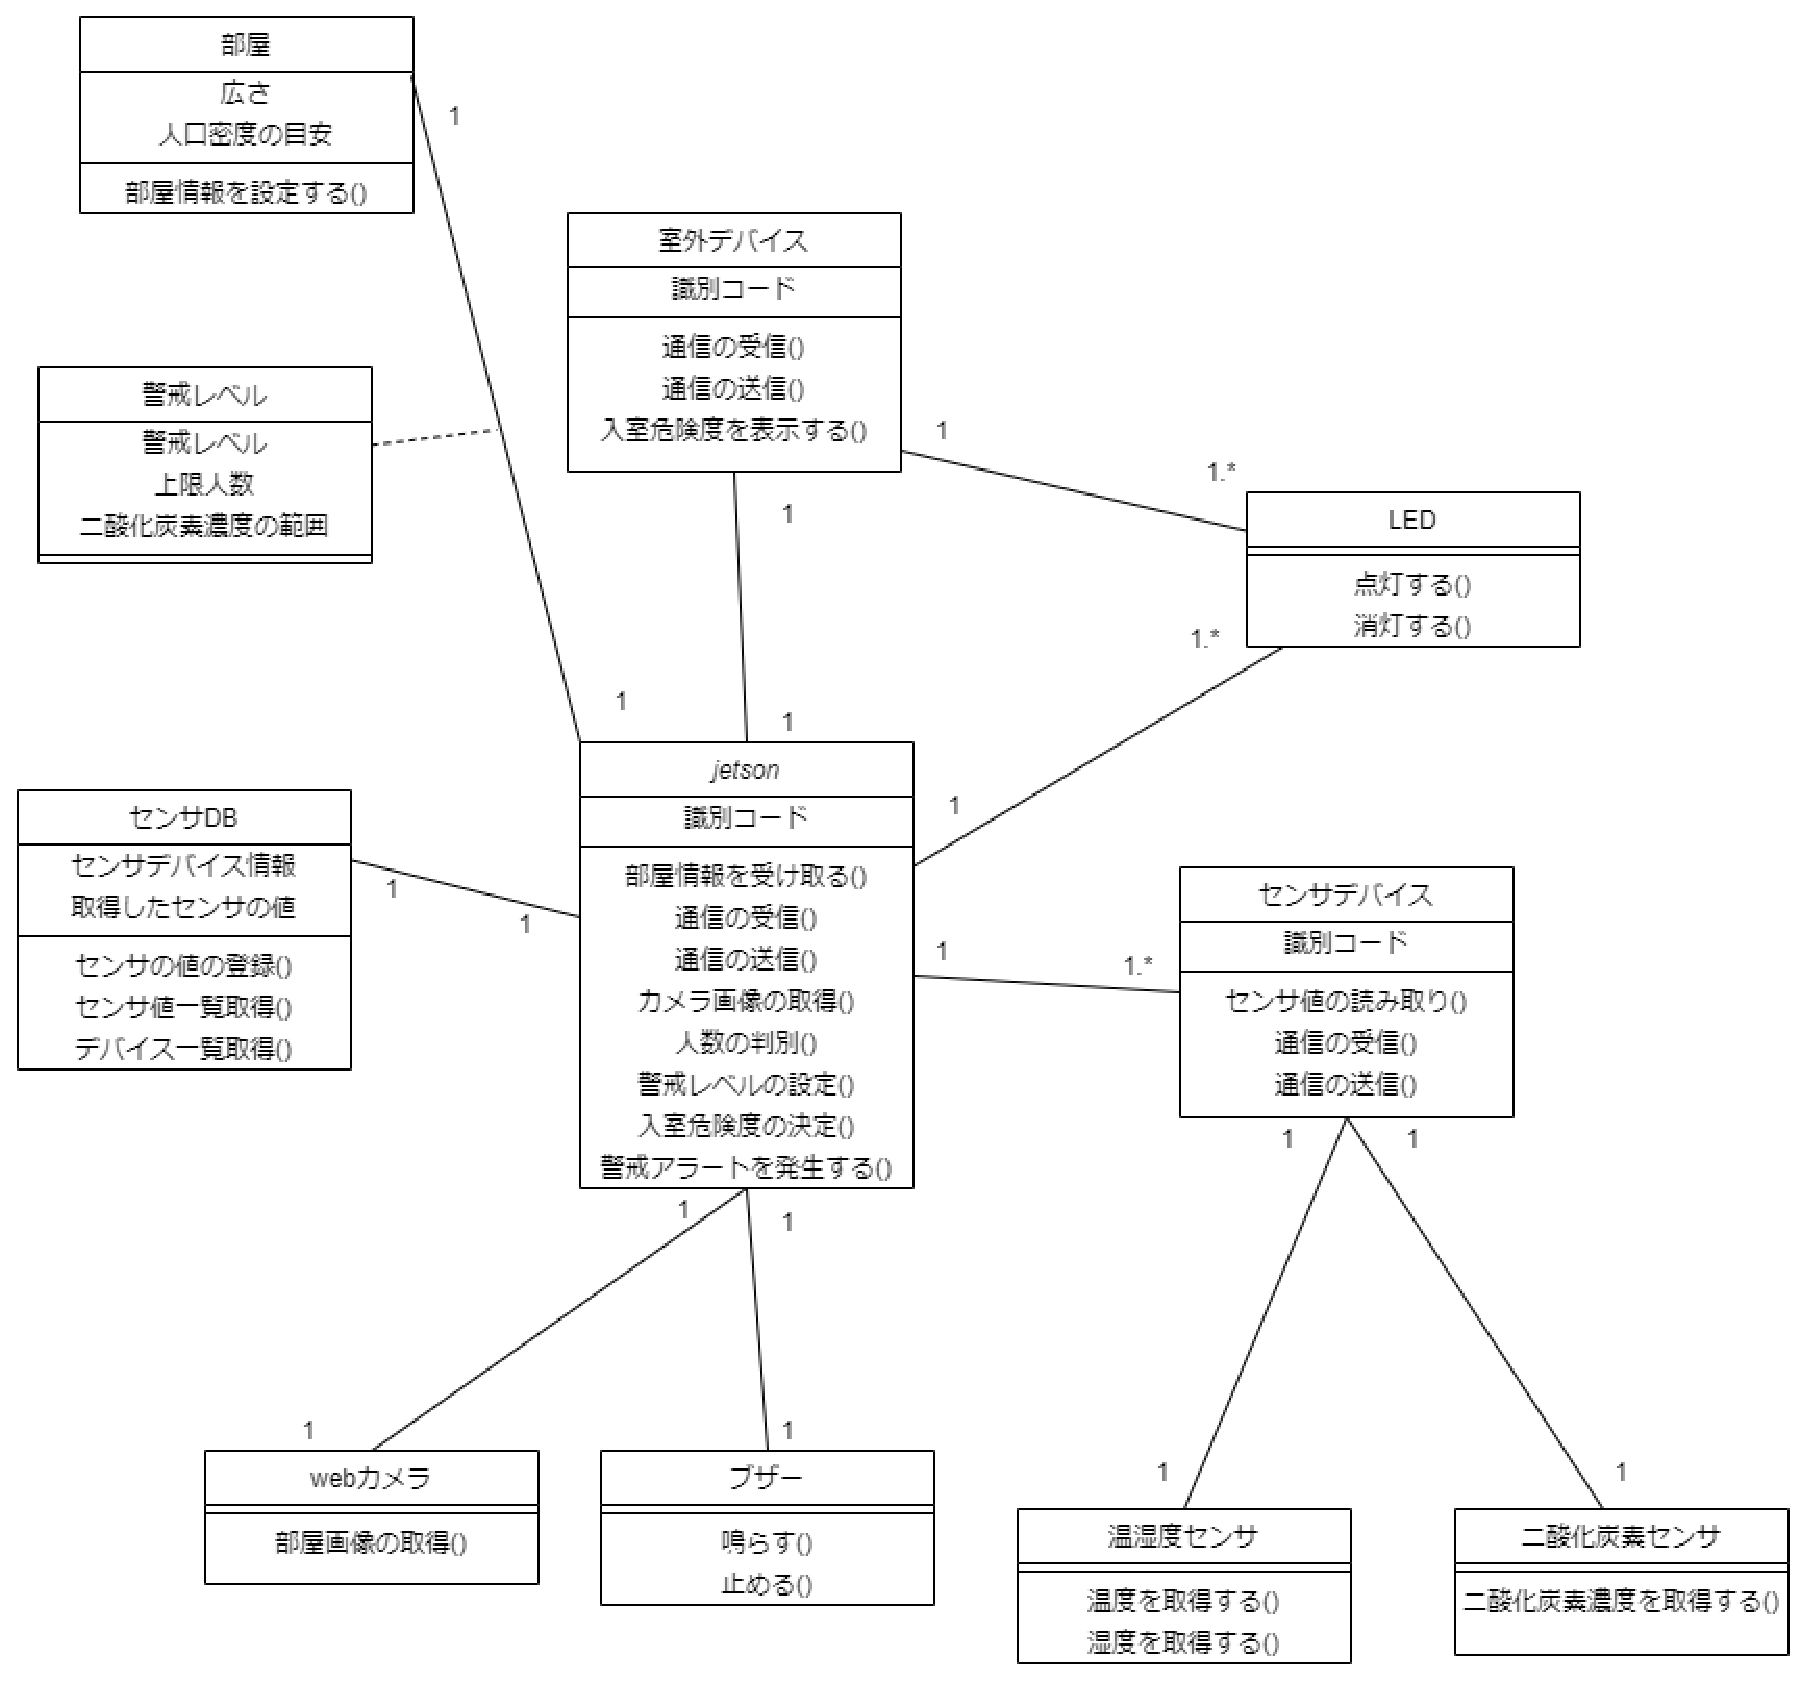
\includegraphics[width=12cm]{class.eps}
	\caption{クラス図}
	\label{class}
\end{figure}


また、以上の基本設計の内容をもとに、結合テスト項目として表\ref{ketugoutest_koumoku}の項目を挙げた。


\begin{table}[H]
	\centering
	\caption{結合テスト項目}
	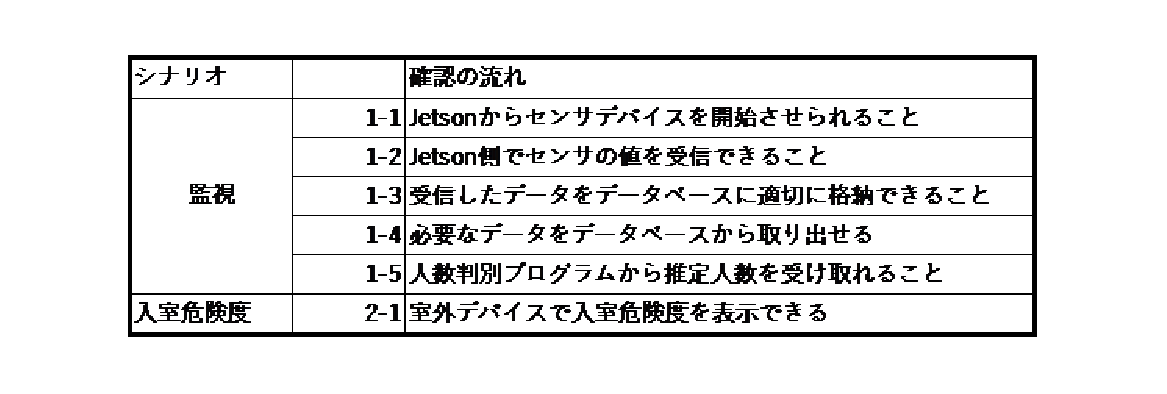
\includegraphics[width=15cm]{ketugoutest_koumoku.eps}
	\label{ketugoutest_koumoku}
\end{table}




	
\section{使用部品の選定(TWELITE)}

基本設計の段階において,筆者が担当した室外デバイスで使用する部品の選定を行った.
室外デバイスのマイコンについては,モノワイヤレス株式会社の無線マイコンであるTWELITEを使用した\cite{twelite}.
室外デバイスはJetsonと通信する必要があり,また,コードの配線を考えずに済むように無線通信ができるマイコンを採用することとした.
さらに設置場所の制約を少なくするため,室外デバイスはできるだけサイズを小さくしたい.このため,マイコンボードに無線機能があらかじめ実装されているもの,乾電池で動作できるものを採用することとした.ただし,乾電池の一般的な起電力である1.5Vで動作するマイコンボードはほとんどないため,ここでは乾電池を2本使用して3Vで動作するものとする.
以上の理由より,起電力3Vで動作し,無線機能があらかじめ実装されているTWELITEを選定した.
今回使用したのはTWELITE DIP BLUEである(図\ref{tweblue}).以下の表\ref{siyou}に仕様を示す.

\begin{figure}
	\centering
	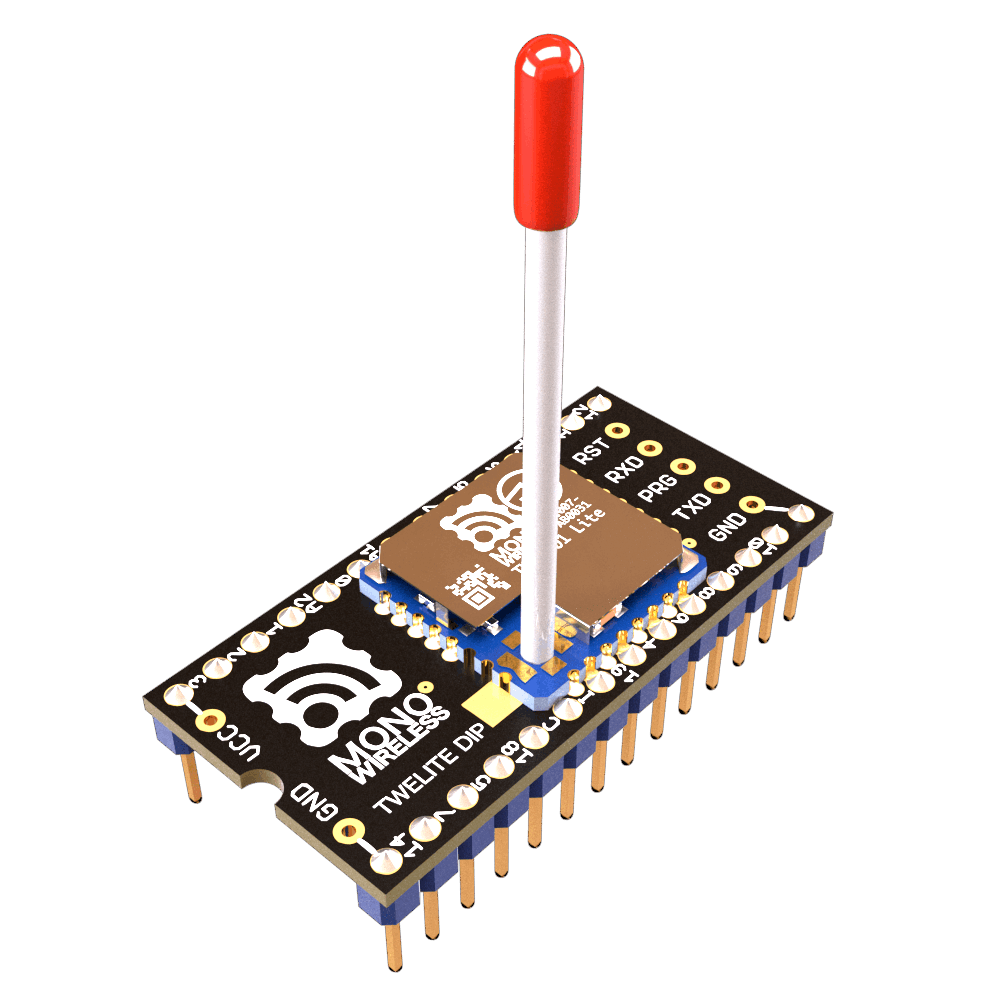
\includegraphics[width=0.3\linewidth]{tweblue}
	\caption{TWELITE DIP BLUE}
	\label{tweblue}
\end{figure}

\begin{table}
	\centering
	\caption{TWELITE DIP BLUEの仕様}
	\begin{tabular}{|c|c|}
		\hline
		送信出力 & +2.50dBm \\
		\hline
		受信感度 & -95dBm \\
		\hline
		送信電流 & 15.3mA (+2.50dBm出力時) \\
		\hline
		受信電流 & 17.0mA \\
		\hline
		外形寸法 & 35.7mm x 17.7mm x 3.5mm \\
		
		& (アンテナ,コネクタ,端子除く) \\
		\hline
		& 3.6g (マッチ棒アンテナ版) \\
		
		重量 & 3.7g (同軸コネクタ版) \\
		
		& (アンテナ,コネクタ,端子除く) \\
		\hline
		動作電圧 & 2.3~3.6V \\
		\hline
		動作温度 & -40~85℃ \\
		\hline
		電波認証 & ARIB STD-T66 (技適) \\
		\hline
	\end{tabular}
	\label{siyou}
\end{table}
\newpage
	%第3章

\section{詳細設計}

オブジェクト間のメッセージのやりとりを時系列に沿って表現するために,以下に示すシーケンス図を作成した.
換気要請についてのシーケンス図を図\ref{sequencekanki}に,室内の監視についてのシーケンス図を図\ref{sequencekanshi}に,室内環境についてのシーケンス図を図\ref{sequenceshitsunai}に,入室危険度についてのシーケンス図を図\ref{sequencenyushitsu}に示す.

\begin{figure}
	\centering
	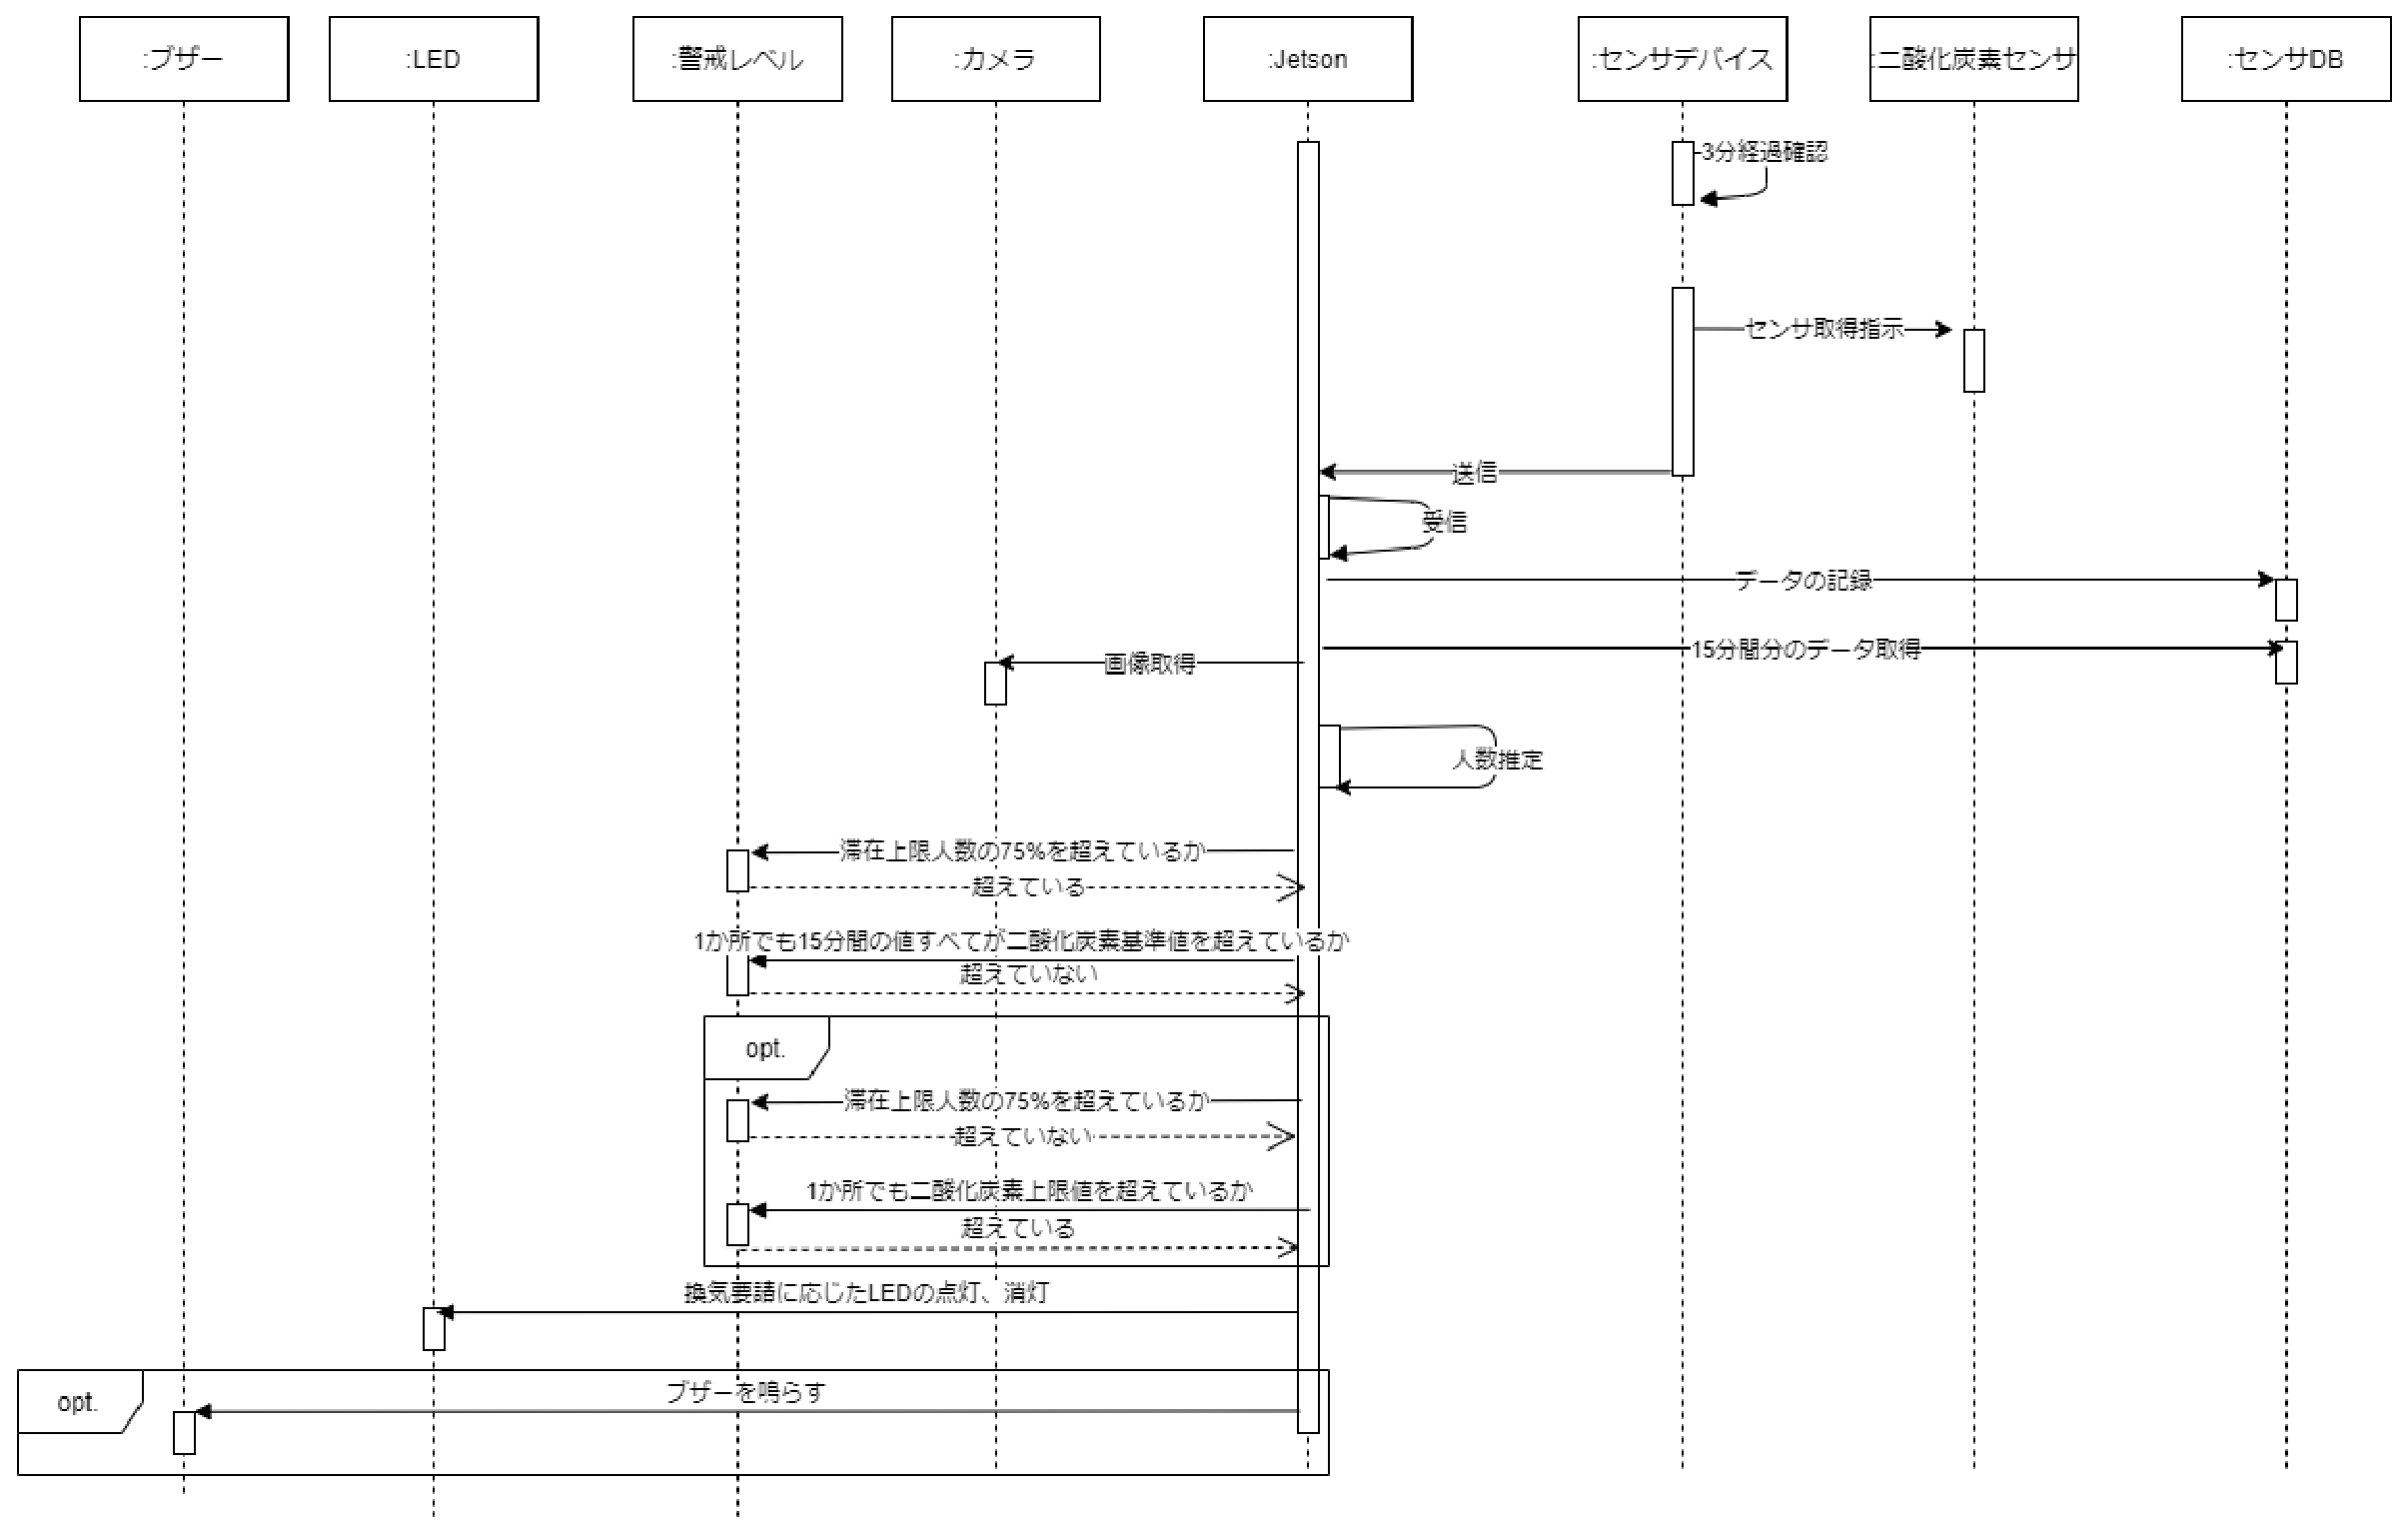
\includegraphics[width=15cm]{./uml/sequence_kanki_2}
	\caption{換気要請についてのシーケンス図}
	\label{sequencekanki}
\end{figure}

「換気要請」について,まずセンサデバイスが3分経過ごとに二酸化炭素センサへ値の取得指示を出す.
取得した二酸化炭素濃度をJetsonへ送信し,Jetsonはセンサデータベースへデータを記録した後,15分間分のデータをデータベースから取得する.
次にカメラから画像を取得し人数推定を行う.推定した人数と取得した二酸化炭素濃度値を,警戒レベルが保有する上限人数と二酸化炭素濃度の基準値と比較し換気要請の判断を行う.その後換気要請に応じてLEDとブザーに指示を出す.

\begin{figure}
	\centering
	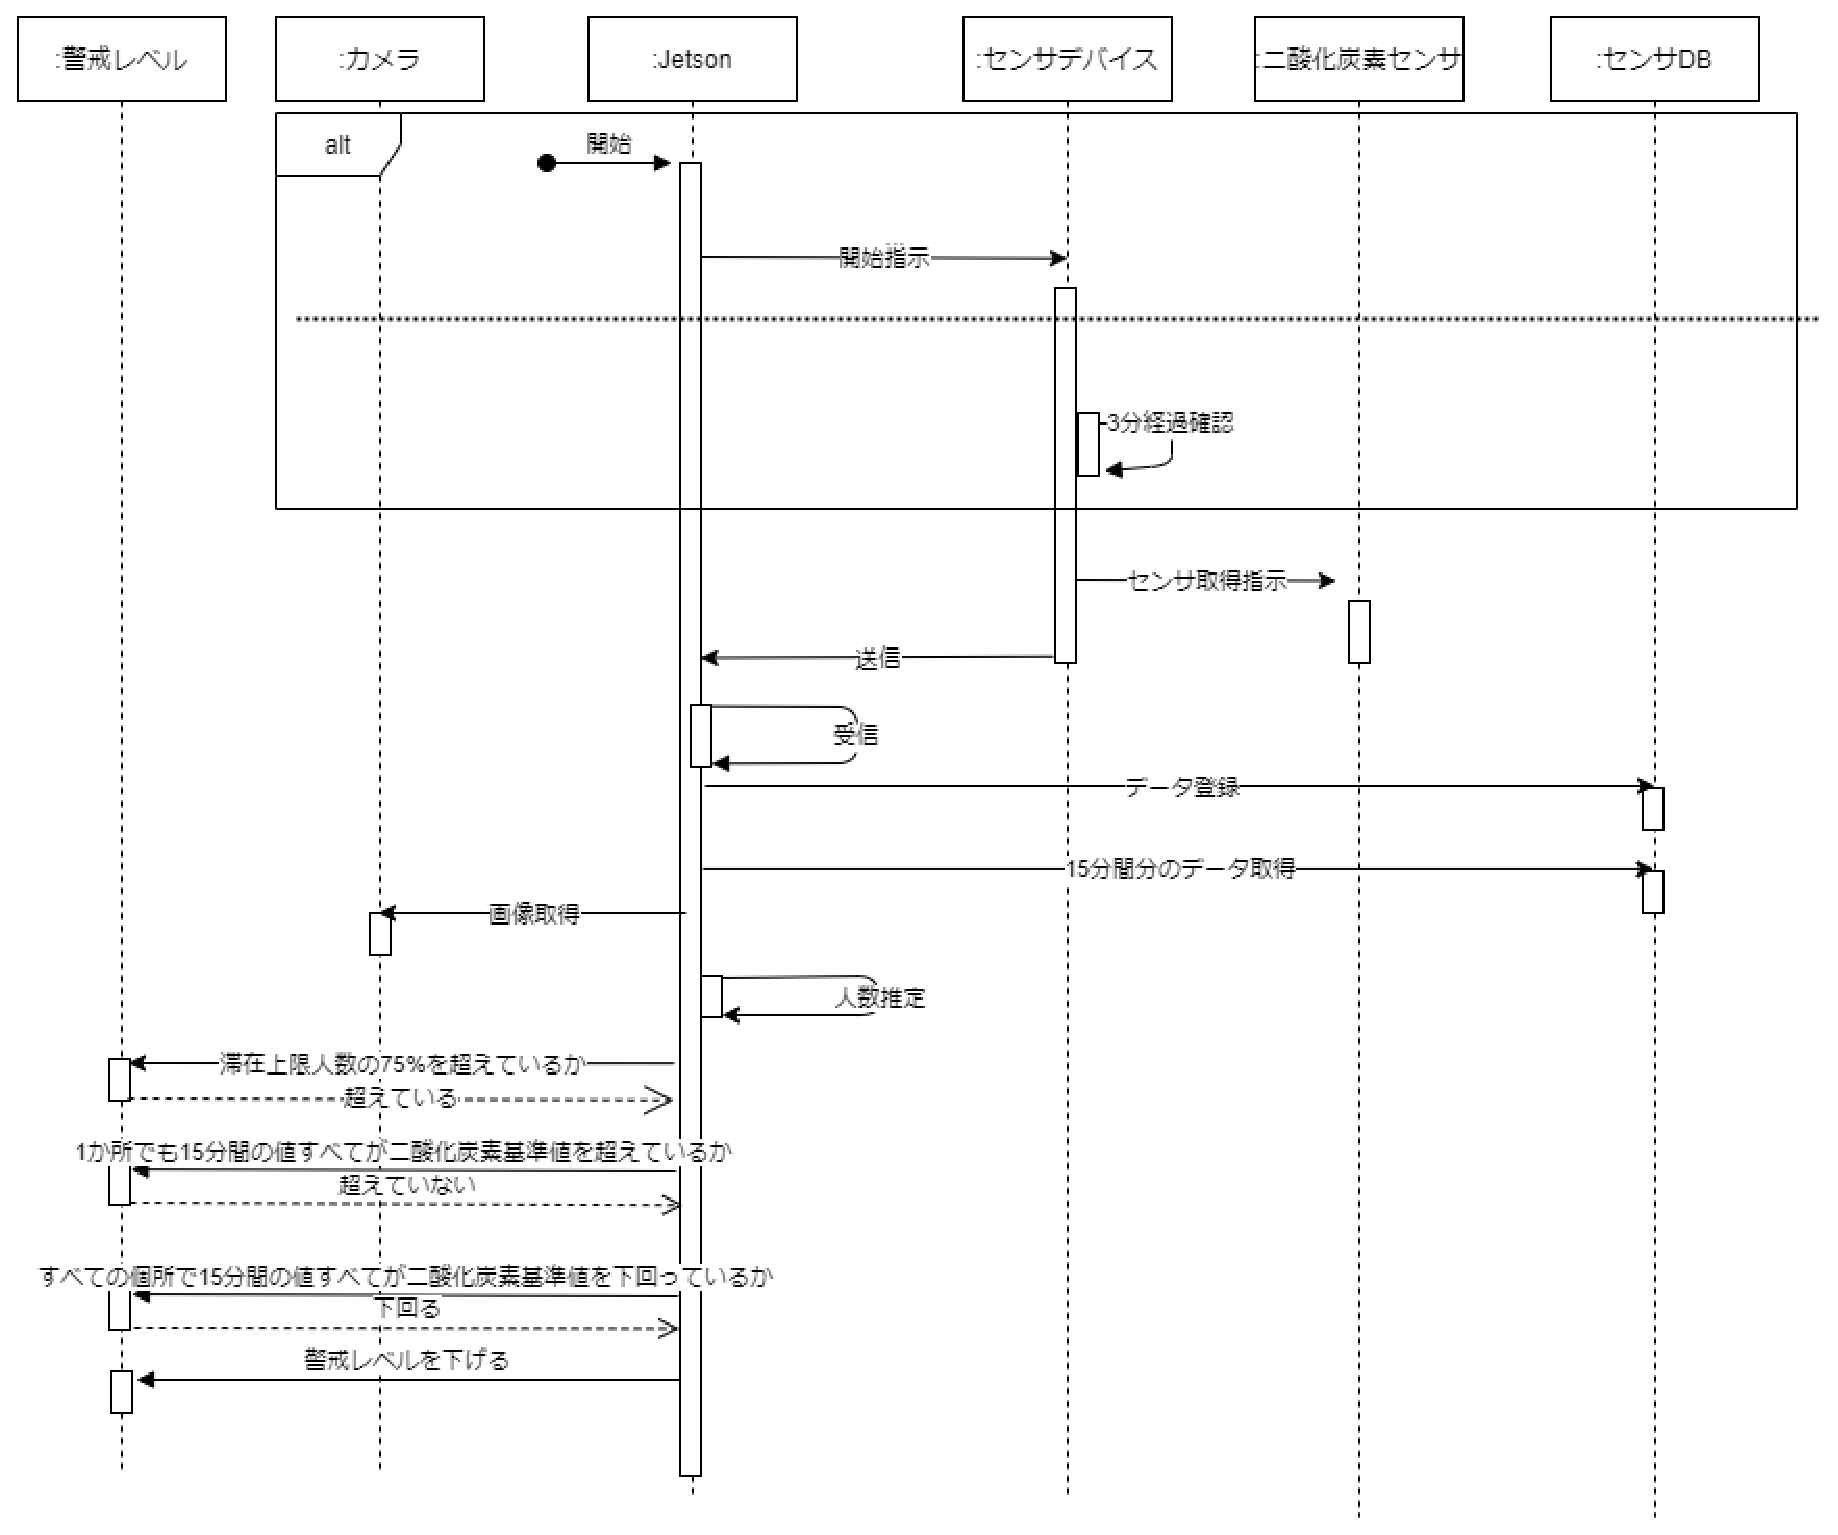
\includegraphics[width=15cm]{uml/sequence_kanshi_3}
	\caption{室内の監視についてのシーケンス図}
	\label{sequencekanshi}
\end{figure}

「室内の監視」について,システムを起動するとJetsonはセンサデバイスへ開始の指示を行う.
指示を受けたセンサデバイスは二酸化炭素センサへ値の取得指示を出す.
その後はセンサデバイスが3分経過ごとに二酸化炭素センサへ値の取得指示を出し,人数推定を行うまで「換気要請」の場合と同様であり,
推定した人数と取得した二酸化炭素濃度値を,警戒レベルが保有する上限人数と二酸化炭素濃度の基準値と比較し,警戒レベルを設定する.

\begin{figure}
	\centering
	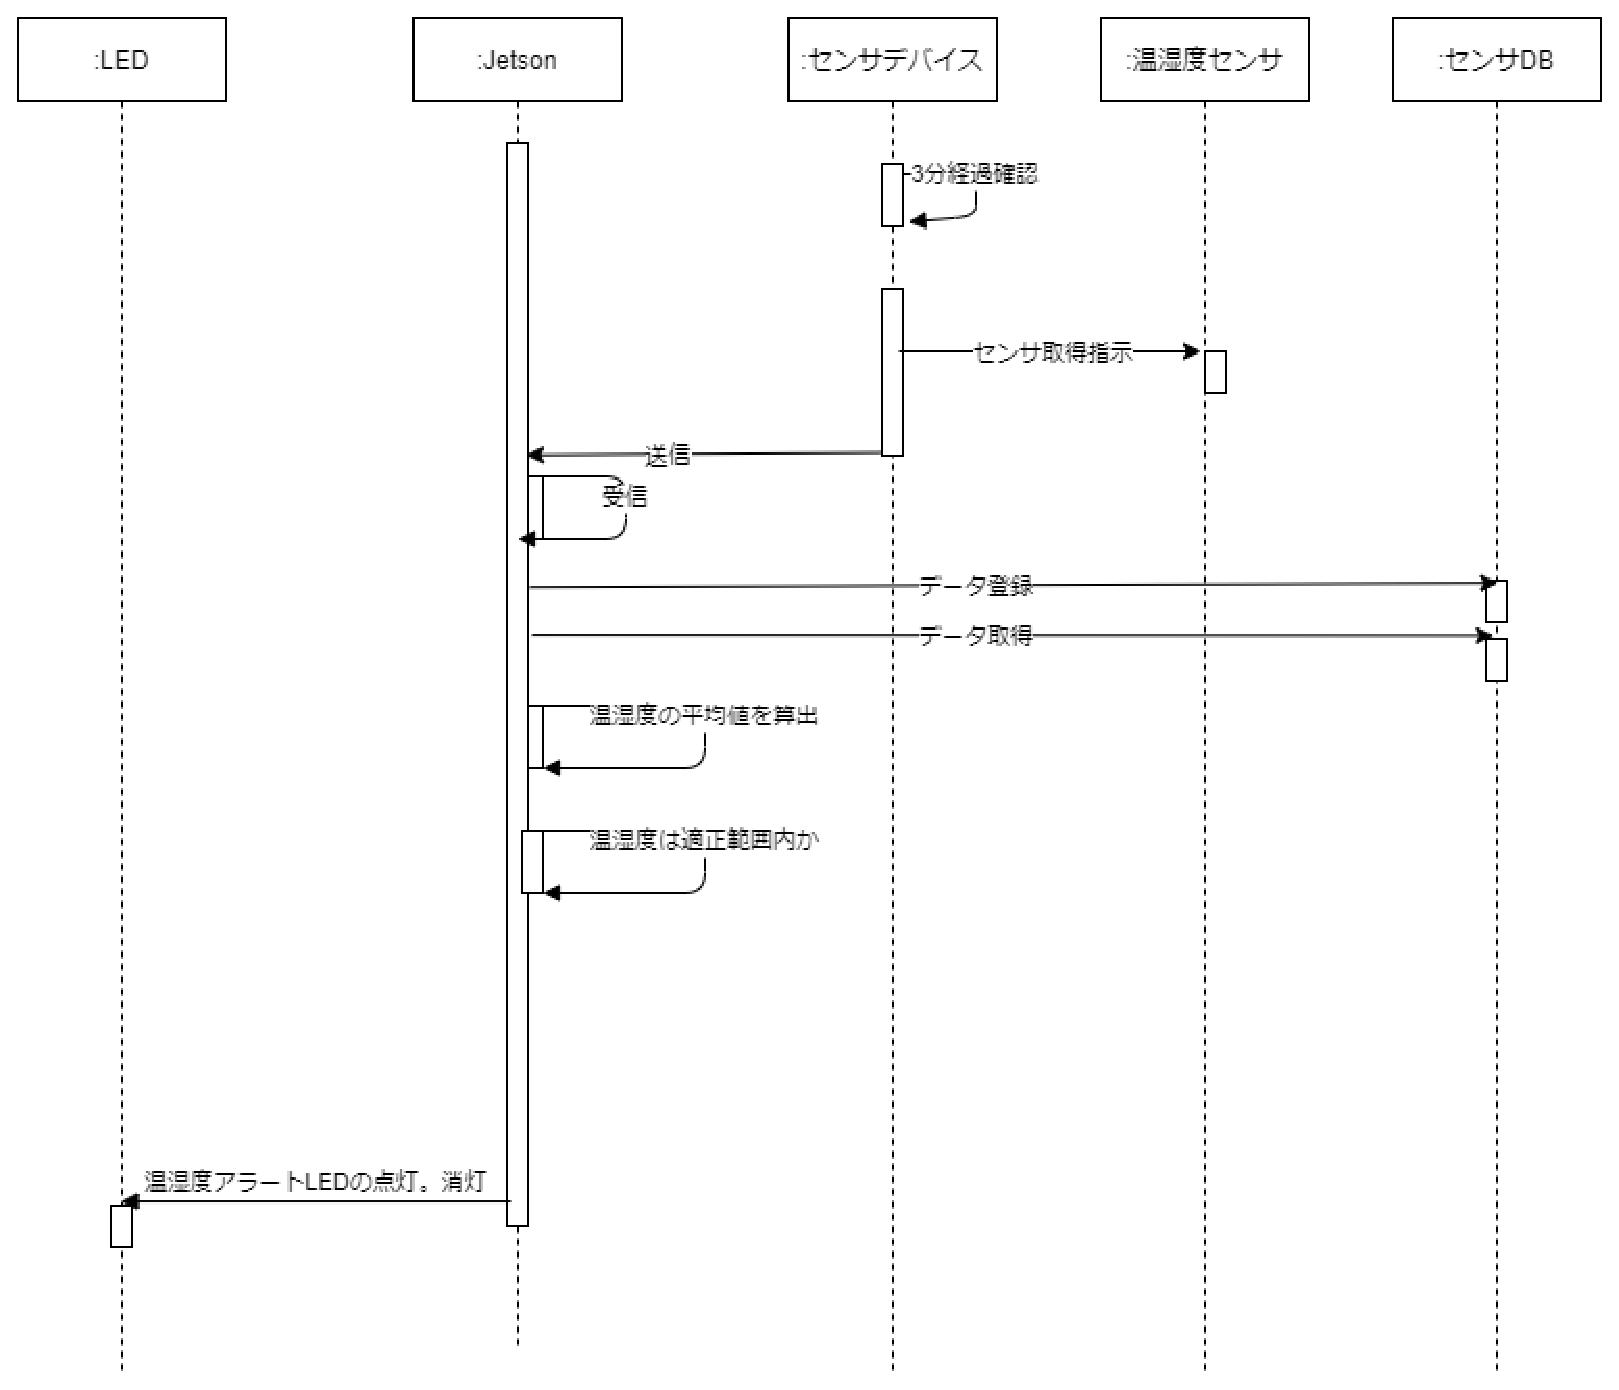
\includegraphics[width=15cm]{uml/sequence_shitsunai_2}
	\caption{室内環境についてのシーケンス図}
	\label{sequenceshitsunai}
\end{figure}

「室内環境」について,まずセンサデバイスが3分経過ごとに温湿度センサへ値の取得指示を出す.
取得した温湿度をJetsonへ送信し,Jetsonはセンサデータベースへデータを記録した後,これまでの温湿度データを取得する.
温湿度の平均値を算出し,適正範囲内か否かによって温湿度アラートLEDを制御する.

\begin{figure}[htbp]
\centering
\includegraphics[width=15cm]{./uml/sequence_nyushitsu_e.eps}
\caption{入室危険度についてのシーケンス図}
\label{sequencenyushitsu}
\end{figure}

「入室危険度」について,人数推定を行うまでは「換気要請」等と同様の流れである.
その後,現在の室内滞在人数と,警戒レベルが保有する滞在上限人数,滞在推奨人数を比較し入室危険度を決定する.
Jetsonから室外デバイスに入室危険度を送信し,室外デバイスは入室危険度に応じてLEDの制御を行う.
赤枠で囲んだ屋外デバイスとLEDは筆者が実装を担当する.

次に,筆者が実装を担当した室外デバイスのステートチャート図を図\ref{statechartokugai}に示す.

\begin{figure}
	\centering
	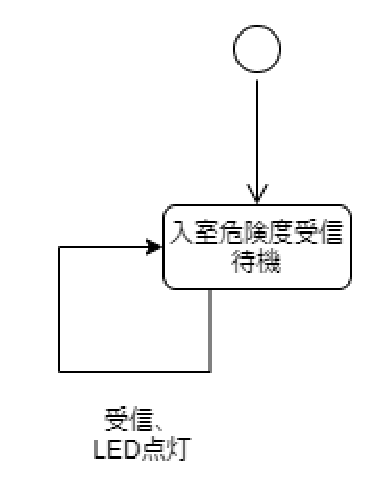
\includegraphics[width=0.3\linewidth]{uml/statechart_okugai_1}
	\caption{室外デバイスのステートチャート図}
	\label{statechartokugai}
\end{figure}

室外デバイスはシステムが稼働している間,常に入室危険度の受信待機状態であり,Jetsonから入室危険度が送られてきた場合に入室危険度に応じた色のLEDが点灯する.

以上の詳細設計より表\ref{tantaitestsitsugaikoumoku}に示す室外デバイスにおける単体テスト項目を挙げた.

\begin{table}
	\centering
	\caption{室外デバイスにおける単体テスト項目}
	\label{tantaitestsitsugaikoumoku}
	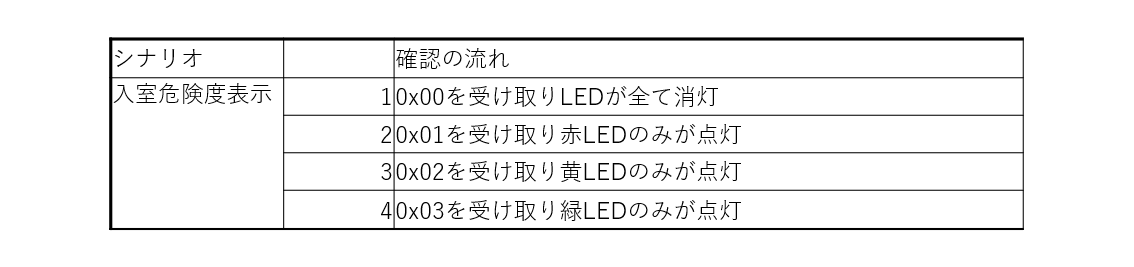
\includegraphics[width=0.9\linewidth]{test/tantaitest_sitsugai_koumoku2}
\end{table}
	
	%第4章
	\chapter{実装・検証}
	%第4章:実験結果・考察
本章ではV字モデルの開発プロセスに従い行った、実装および検証について説明する。4.1節では、各設計に基づいて行った実装について説明し、4.2節では単体テスト、結合テスト、総合テストの実施について説明する。
	%第4-1章:実装

\section{実装}

第3章で述べたシステム全体の機能はグループで実装を行い,筆者は室外表示用のデバイスの実装を担当した.
室外デバイスの動作としては,Jetsonから入室危険度を受信し,入室危険度に応じたLEDの制御を行うというものである.
また,第3章でも述べたように,無線マイコンとしてTWELITEを用いて実装を行った.
マイコンボード上で動作するソフトウェアについては,TWELITE MWX ライブラリを利用し,C++言語を用いて開発を行った.
図\ref{zikki}が実際に作成した室外デバイスである.

\begin{figure}
	\centering
	\includegraphics[width=0.5\linewidth]{zikki}
	\caption{作成した室外デバイス}
	\label{zikki}
\end{figure}

筆者が担当する室外表示デバイスに対して単体テストを行った.その後,グループメンバーが開発した機能部と合わせて結合テストと総合テストを行った.以下,検証項目について述べる.
	%第4章:検証

\section{検証}

\subsection{単体テスト}

詳細設計の際に挙げた単体テストの項目に従って単体テストを行った.単体テストの結果を表\ref{tantaitestsitsugaikekka}に示す.

\begin{table}
	\centering
	\caption{室外デバイスの単体テストの結果}
	\label{tantaitestsitsugaikekka}
	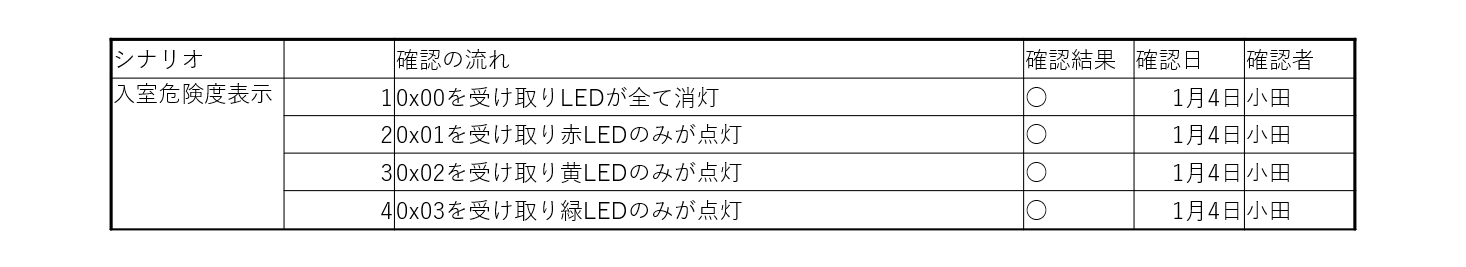
\includegraphics[width=0.9\linewidth]{test/tantaitest_sitsugai_kekka2}
\end{table}

単体テストの実施においては,TWELITEのUART接続を用いてデバイスをPCに接続して行った.
単体テスト項目1~4までPC上から室外デバイスにコマンドを送り,すべて消灯した状態と各入室危険度を表すLEDの制御が正しくできることを確認した.

\subsection{結合テスト}

基本設計の際に挙げた結合テストの項目に従って結合テストを行った.結合テストの結果を表\ref{ketugoutest}に示す.

\begin{table}
	\centering
	\caption{結合テストの結果}
	\label{ketugoutest}
	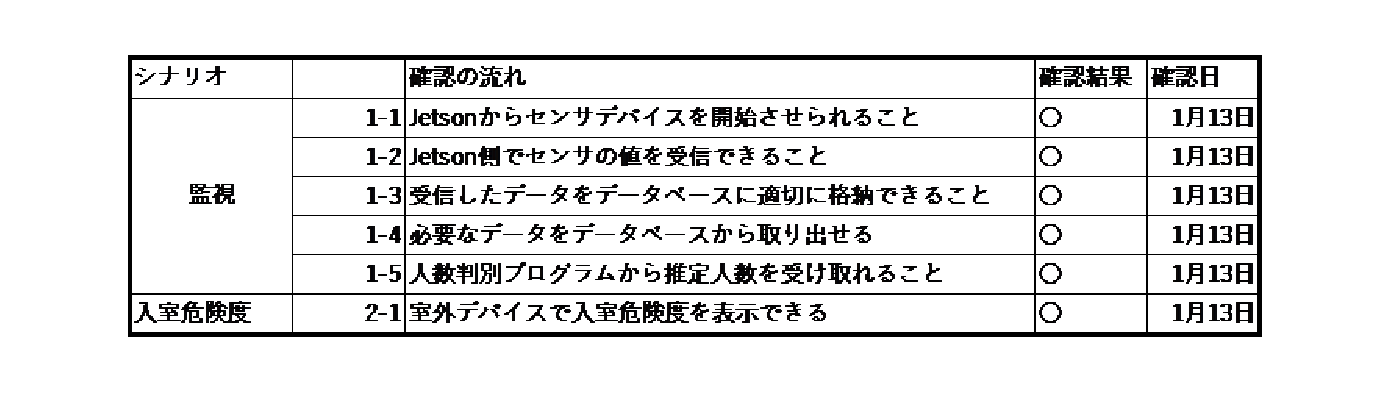
\includegraphics[width=0.9\linewidth]{test/ketugoutest}
\end{table}

結合テストは,環境値評価と人数推定を同一プログラムで行える状態で,データベース操作のプログラムも同一のJetsonで行えるようにして状態で実施した.

項目1-1については,センサデバイスの電源が入っている状態でJetsonの処理プログラムを開始したところ,LEDの状態変化によりセンサデバイスが正しく動作することを確認した.
項目1-2については,Jetsonの処理プログラムを実行することでセンサデバイスから電波を受信していることを確認した.
項目1-3については,処理プログラムの動作中にデータベースに格納された値を定期的に確認し,受信したデータを適切に格納できていることを確認した.
項目1-4については,データベースにデータが格納されている状態から,その値を用いた評価ができていることを確認した.
項目1-5については,プログラムの中で人数推定の結果を正しく受け取れていることを確認した.
項目2-1については,Jetson上で評価した入室危険度に応じて室外デバイスのLEDが正しく点灯していることを確認した.

\subsection{総合テスト}

要求定義の際に挙げた総合テストの項目に従って総合テストを行った.総合テストの結果を表\ref{sougoutest}に示す.

\begin{table}
	\centering
	\caption{総合テストの結果}
	\label{sougoutest}
	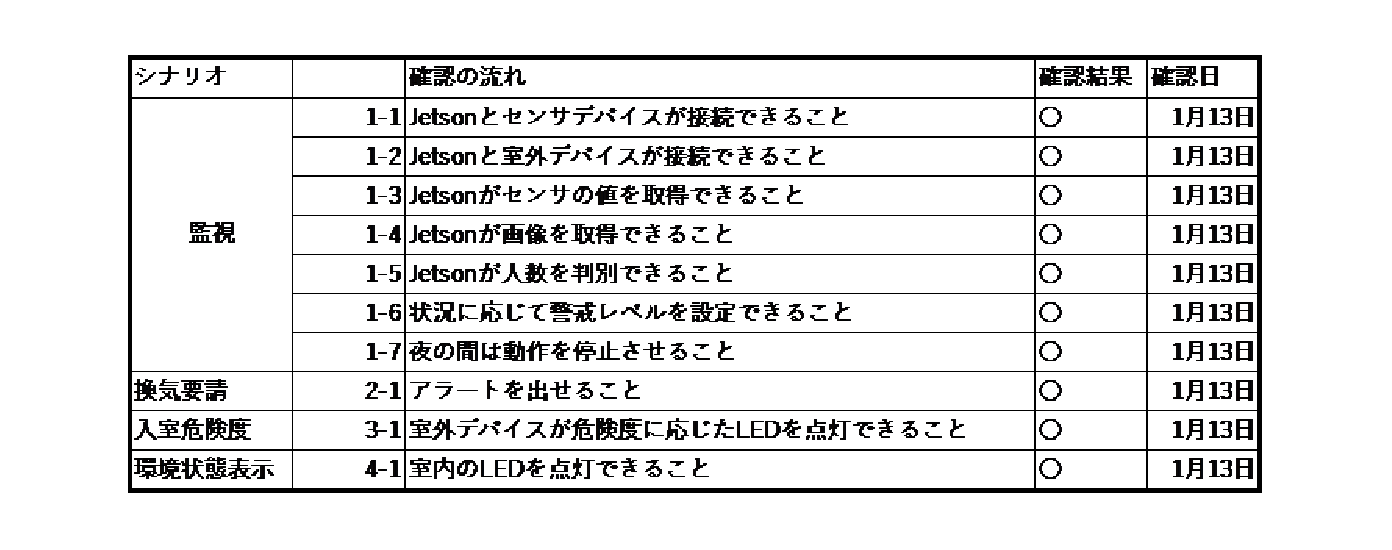
\includegraphics[width=0.9\linewidth]{test/sougoutest}
\end{table}

総合テストは実際にシステムの利用を想定した環境で行った.
項目1-1については,システム実行時にセンサデバイスがJetsonからの開始信号を受け取ることでLEDの状態が変化し,Jetsonとセンサデバイスが接続できていることを確認した.
項目1-2については,システム実行時に室外デバイスのLEDがすべて消灯されるようにすることで,Jetsonと室外デバイスが接続できていることを確認した.
項目1-3については,Jetsonがセンサデバイスから値を受信し,その後の処理に利用できていることを確認した.
項目1-4については,JetsonがWebカメラから画像を取得し,その画像をJetsonと接続したPC上に表示することで正しく画像が取得できていることを確認した.
項目1-5については,人数の異なる集合写真を用いて人数推定を行い,おおむね正しく人数判別できていることを確認した.
項目1-6については,人数の多い集合写真を用いて,室内滞在人数が多く,二酸化炭素濃度値が基準値より高い場合に警戒レベルが上がっていることを確認した.
同様にして,項目2-1と項目4-1について,換気要請のブザーや室内LEDが正しく動作することを確認した.
項目1-7については,設定した時間中,センサ値の取得およびシステムの処理が中断されることを確認した.
項目3-1については,Jetsonが評価した入室危険度に応じて室外デバイスのLEDが正しく点灯することを確認した.
	
	%第5章
	\chapter{評価・考察}
	%第5章
本章では、本システムに対する評価・考察を行い、今後の課題や将来性についても述べる。

まず3.1節に挙げた、本システムが果たすべき2つの大きな役割に対して評価する。3.1節において、本システムが果たすべき役割について、「感染症予防対策のルールを守ってもらうよう働きかける役割」、「感染症予防対策の基準を定める役割」の2つを挙げた。感染症予防対策のルールを守ってもらうよう働きかける役割については、室内環境に応じた換気要請の発出や、感染リスクのレベルの通知によって、換気や人数調整といった具体的なアクションを促すことが実現できていると考えられる。感染症予防対策の基準を定める役割については、利用者が感染症予防のためにとるべき、換気と部屋に滞在する人数の調整というアクションについて、感染症予防の観点から、部屋を安全な状態に保つため、具体的にその基準を定めることで、利用者自身が感染症予防のためにとるべきアクションを明確にすることが実現できていると考えられる。

また本システムでは、センサデバイスで取得したデータを随時データベースに記録しているほか、室内の滞在人数や警戒レベル、感染リスクといったデータも、センサデバイスからのデータ更新に伴って導き出されていることから、必要に応じてデータを保管しておくことで、システム外部で様々なデータの相関を調べることもできる。そのため、感染症予防対策の基準を定める役割に関しては、応用の余地があると考えられ、例えば以下のような応用の仕方が考えられる。

本システムでは、分析に活かせる多くのデータを導き出せるが、中でも設計の段階から分析に役立てられるデータとして着目していたのは、警戒レベルと感染リスクのデータである。既に述べたように、室内にある程度の人数が滞在していないと警戒レベルの導出は行われない。そのため警戒レベルの推移のデータは、その部屋が警戒レベルを導出できる条件下で利用されているとき、どの程度二酸化炭素濃度が高まりやすいかを確認でき、運用ルール改定の基準にできる。また、警戒レベルと感染リスクのデータをシステム内部で分析し、本システムでは固定的である、二酸化炭素濃度と警戒レベル、警戒レベルと滞在可能人数の関係を、部屋の警戒レベルと感染リスクの変動の仕方に応じて流動的に変化させると、よりその部屋にあった感染症予防対策を講じることが可能になると考えられる。

感染リスクのデータは、換気状況など、部屋の運用の仕方が適切であるかどうかを示しているため、部屋が感染症予防対策上、危険な状態で使用されていないかを確認できる。そのため学校やオフィス、公共施設などでの利用のケースを想定すると、時間帯ごとの感染症予防対策への取り組みの徹底度合いが、エビデンスとして残されることから、管理者側からの適切な指導が行えるほか、各部屋の責任者となる者が、感染症予防対策に、より注意して取り組むことができると考える。

本システムの設計時の着想では、利用環境ごとに異なる、床面積の広さ・空間の広さ、換気のしやすさや窓の位置と数、換気設備の有無、部屋利用者の活動の仕方などに柔軟に対応し、利用環境に合わせた感染症予防対策の基準を定め、利用者に感染症予防対策のルールを守ってもらうよう働きかけられることが本システムの特徴であった。実際に、本システムは4.2節の総合テストでの検証のように、様々なシナリオにあった感染症予防の働きかけが可能となることが考えられる。しかしながら、本システムでの感染症予防対策の基準の決め方では、換気のしやすさや、部屋の床面積の広さのわりに、ものが多く置かれているなどの理由から実際の空間が狭いというような部屋の特性が、そのまま二酸化炭素濃度の上昇の仕方に反映されることを前提としている部分があり、柔軟性に欠けていると考える。理想的な環境における本システムの実用性は確認されたものの、部屋ごとの特性を加味した感染症予防対策の基準を、実際の利用環境において適切に定めるためには、本システムでの室内環境の分析の仕方よりも複雑に、室内環境を分析する必要があるとも考えられ、部屋の特性自体をシステムの分析機能によって導き出すことができると、現在のシステムと比較し、よりその部屋の特性に適合した感染症予防対策の基準の設定を行うことができるため、更なる研究と改良の余地が大いに残されていると考える。



	%第5-1章:評価

\section{評価}

第3章では,感染症予防サポートシステムは,感染症予防の観点から感染リスクのレベルを通知するとともに,感染リスクを軽減する環境づくりをサポートするという目的を基にして,下記の2点の要求事項を満たす必要があるとした.

\begin{itemize}
	\item 室内環境が測定できること.
	\item 設定した感染リスクの基準に従って通知ができること.
\end{itemize}

「室内環境が測定できること」という要求事項に関して,作成したシステムは二酸化炭素濃度,温湿度,室内滞在人数の測定ができるため,要求を満たすことができたといえる.
「設定した感染リスクの基準に従って通知ができること」という要求事項に関しては,警戒レベル,換気要請の基準,入室危険度を設定し,警戒レベルおよび入室危険度はLED,換気要請はブザーによって,ユーザーに感染リスクの情報を,視覚や聴覚で分かりやすく能動的に通知することができた.室外のユーザーには室外デバイスによるLEDでの入室危険度の通知,室内のユーザーにはブザーとLEDによる換気要請や警戒レベルの通知というように,対象とするユーザーによって提供する情報,提供の方法を変えることで,室内外から共に感染リスクを軽減する環境づくりをサポートするシステムとなった。
	%第5章:考察

\section{考察}

今回作成した感染リスク通知デバイスは3色のLEDで入室危険度を分かりやすく表示するというものである.
理想的には,センサーとカメラで収集した施設内の環境情報(在室人数,入室できる人数,二酸化炭素濃度水準,換気状態,感染リスク等の情報)を利用者対象別に提供することが望ましいが,ハードや時間の制約のために,室内外への感染リスクに関する基本的な情報提供機能のみの実装となり,すべての環境情報をユーザーに知らせるまで至らなかった.
しかしながら,在室人数,入室可能人数,二酸化炭素濃度等の数値に関して,本システムはデータを収集できている.
今後,ディスプレイ等を使用すれば,Jetsonから各種データを受け取ることで室内外により詳細な環境情報を表示することができると考える.

	
	%第6章
	\chapter{あとがき}
	%あとがき
本研究ではセンシング技術、物体検出技術、および複数デバイス間の無線通信という3つの技術とデータ分析の組み合わせによって、感染症予防という、研究・実用化が活発に進められる分野において新たな価値を生み出すことができた。感染症予防に関しては、既に様々な分野で研究・開発がなされているものと思われるが、今回私たちが開発したシステムも、感染症予防の取組を援用するシステムとして貢献できると考える。

また今回の研究では、感染症予防のために活用できるシステムの社会的な必要性が高まり、多くの企業や研究機関により研究・開発が進められている状況下で、感染症予防のために用いるシステムとして、3 密回避に役立てられるという、新型コロナウイルスの世界的な流行以前にはなかった新しい価値を持たせることも、1つの目標として定められた。本研究において、私たちの考える感染症予防のサポートシステムの基本形を提案することができた。今後さらなる研究が進められれば、より高いリアルタイム性と精度を併せ持つモニタリングと、感染症予防対策基準の設定機能における更なる柔軟性を実現でき、より利用しやすいものへと改良が進められることから、拡張性のある研究であると考える。

	%--ここまで本文--
	
	
	%謝辞
	\newpage
	\addcontentsline{toc}{chapter}{\protect\numberline{謝辞}{}}
	\chapter*{謝辞}
	%--ここから謝辞--
	本研究を進めるにあたり,懇篤な御指導,御鞭撻を賜わりました本学高橋寛教授に深く御礼申し上げます.
	
	本論文の作成に関し,詳細なるご検討,貴重な御教示を頂きました本学甲斐博准教授ならびに王森レイ講師に深く御礼申し上げます.
	
	本研究に際しご審査いただきました稲元 勉講師,井門 俊講師に深く御礼申し上げます.
	
	最後に,多大な御協力と貴重な御助言を頂いた本学工学部情報工学科情報システム工学講座高橋研究室の諸氏に厚く御礼申し上げます.
	
	%--ここまで謝辞--
	
	%参考文献
	\begin{thebibliography}{99}
		%ここから参考文献
		
		\bibitem{qa}
		厚生労働省,新型コロナウィルスに関するQ\&A(一般の方向け)$|$厚生労働省,
		https://www.mhlw.go.jp/stf/seisakunitsuite/bunya/kenkou\_iryou/\\dengue\_fever\_qa\_00001.html,2021-1-4
		
		\bibitem{kanki}
		厚生労働省,「換気の悪い密閉空間」を改善するための換気の方法,
		https://www.mhlw.go.jp/content/10900000/000618969.pdf,2020-4-3
		
		\bibitem{isence}
		中畑和之,森伸一郎,板垣吉晃,河合慶有, "コロナウイルス対策のための教室換気実験とアラートシステムの構築," 愛媛大学工学部社会基盤iセンシングセンター報告資料,  2020年11月.
		
		\bibitem{vji}
		V字モデル(V-model)とは -IT用語辞典 e-Words,
		https://e-words.jp/w/V%E5%AD%97%E3%83%A2%E3%83%87%E3%83%AB.html
		
		\bibitem{uml}
		株式会社 オージス総研, かんたんUML[増補改訂版], 翔泳社, 2003
		
		\bibitem{twelite}
		モノをつなぐ無線マイコンモジュール TWELITE-トワイライト - MONO-WIRELESS.COM,
		https://mono-wireless.com/jp/products/TWE-LITE/index.html
		%ここまで参考文献
		
	\end{thebibliography}
\end{document}
